

\section{Beyond Standard Model for Lepton Universality Violation}
\label{sec:relatedWorks:bsm}

The primary signal used in our $B(W\to l \nu )$ measurement is \ttbar process. If any beyond standard model (BSM) leads to a small amount of lepton universality violation (LUV) in the top decay, it will be observed as a non-universality of $B(W\to l \nu )$ in our analysis. Besides mediating top quark decay, it is possible for the BSM to affect the experimental observables in other ways. For example, BSM particle X could be produced on-shell in association with t and b quark in the t-channel $pp \to t b X$, where X is usually at TeV scale and induces LUV. In this circumstance, the heavy on-shell X decay gives rise to highly boosted leptons.  However, since our $B(W\to l \nu )$ measurement is primarily based on the trailing leptons in the dilepton channels and low energy taus in the lepton-plus-tau channels, the observables in our analysis are insensitive to such scenario. Thus when estimating the sensitivity of our measurement to BSMs, we focus on the LUV effect in the top decay. 

\begin{figure}[ht]
    \centering
    % Using the layered layout
    \feynmandiagram [layered layout, small,horizontal=a to b] {
      a [particle=\(t\)] -- [fermion] b -- [fermion] f1 [particle=\(b\)],
      b -- [red, boson, edge label'=\(W'\)] c,
      c -- [anti fermion] f2 [particle=\(\nu_{\tau}\)],
      c -- [fermion] f3 [particle=\(\tau\)],
    };\qquad
    \feynmandiagram [layered layout, small,horizontal=a to b] {
      a [particle=\(t\)] -- [fermion] b -- [fermion] f1 [particle=\(b\)],
      b -- [red, scalar, edge label'=\(H^-\)] c,
      c -- [anti fermion] f2 [particle=\(\nu_{\tau}\)],
      c -- [fermion] f3 [particle=\(\tau\)],
    };\qquad
    \feynmandiagram [layered layout, small,horizontal=a to b] {
      a [particle=\(t\)] -- [fermion] b -- [fermion] f1 [particle=\(\nu_{\tau}\)],
      b -- [red, scalar, edge label'=\(LQ\)] c,
      c -- [anti fermion] f2 [particle=\(b\)],
      c -- [fermion] f3 [particle=\(\tau\)],
    };
    \caption{BSMs that could enhance the tau channel in the top decay. }
   \label{fig:relatedWorks:bsm:topdecayBSM}
\end{figure}

The BSMs, which can cause LUV in the top decay, are shown in the Figure~\ref{fig:relatedWorks:bsm:topdecayBSM}. These models include but not are limited to the \PWpr with a non-universal gauge coupling, $H^+$ in the 2HDM, and leptoquark or LQ in many grand unification models. The mechanism for inducing LUV in these BSMs are different: for \PWpr, the coupling to the third generation lepton is elevated by the underline structure of the gauge symmetry extension; for $H^+$, the coupling to tau is stronger due to tau's heavier mass comparing with electron and muon; for leptoquark, LQ can be generation-conserved and thus the third generation LQ from the top decay tends to produce the third-generation fermions. This section first defines the model-independent top decay kinematics, followed by a QFT calculation of the SM top decay width. Then it discusses the three LUV BSMs in Figure~\ref{fig:relatedWorks:bsm:topdecayBSM} and estimates the sensitivity of our $B(W\to l \nu )$ measurement to these BSMs.



\subsection{Kinematics of Top Decay}
\label{sec:relatedWorks:bsm:kinematics}

\begin{figure}[ht]
    \centering
    % Using the layered layout
    \feynmandiagram [layered layout,horizontal=a to b] {
      a [particle=\(t:\, u_a(p_a)\)] -- [fermion] b -- [fermion] f3 [particle=\(b: \,\bar{u}_3(k_3)\)],
      b -- [boson, edge label=\(W^+\), momentum'=\(q\)] c,
      c -- [fermion] f2 [particle=\(\nu_{\tau} :\, \bar{u}_2(k_2)\)],
      c -- [anti fermion] f1 [particle=\(\tau ^+ :\, v_1(k_1)\)],
    };
    \caption{Top decay in the SM.}
    \label{fig:relatedWorks:bsm:topdecaySM}
\end{figure}

Figure~\ref{fig:relatedWorks:bsm:topdecaySM} shows the tree-level diagram of the SM top decay. The incoming top quark is denoted as a u-type spinnor $u_a(p_a)$ with four-momentum $p_a$; the outcoming anti-tau is denoted as a v-type spinnor $v_1(k_1)$ with four-momentum $k_1$; the outcoming  $\nu_\tau$ and $b$ are represented by the $\bar{u}$-type spinnors $\bar{u}_2(k_2)$ and $\bar{u}_3(k_3)$ with four-momentum $k_2$ and $k_3$, respectively. Note that this correspondence between the spinnors $\{ \bar{u}_2(k_2), \bar{u}_3(k_3)\}$ and particles $\{\nu_\tau,b\}$ are the same when \PWpr or $H^+$ mediates the top decay, but are swapped for the leptoquark. The four-momentum exchanged between the fermion currents is denoted as $q=k-1+k_2 = p_a - k_3$. Using the spinnor representation in Figure~\ref{fig:relatedWorks:bsm:topdecaySM}, the pair-wised inner products of the four-momentums in the center-of-mass frame can be calculated based on the energy-momentum conservation:
\begin{equation}
\begin{split}
	q^2 &=  m_t^2 + m_3^2  -2 m_t E_3  \\
    p_a \cdot k_1 &= m_t E_1 \\
    p_a \cdot k_2 &= m_t^2  -m_t E_3-m_t E_1  \\
    p_a \cdot k_3 &= m_t E_3 \\
    k_1 \cdot k_2 &= m_t^2/2 - m_1^2/2 + m_3^2/2 - m_t E_3 \\
    k_2\cdot k_3 &=  m_t^2/2 + m_1^2/2 - m_3^2/2 + m_t E_1 \\
    k_1\cdot k_3 &=   -m_t^2/2 - m_1^2/2 - m_3^2/2 + m_t E_1 + m_t E_3 ,
\end{split}
\label{eqn:relatedWorks:bsm:innerProduct}
\end{equation}

\noindent where all terms related to $m_2$ are neglected because neutrino is massless, and all the inner products are represented in terms of $ ( E_1,E_3 )$ with mass constants. It is equivalent to use $ ( E_2,E_3 )$ or $ ( E_1,E_2 )$ as variables. The top total width is proportional to the integral of the matrix element $\overline{ |\mathcal{M}|^2 } $ over the three-body decay phase space $PS_3$
\begin{equation}
	\Gamma = \frac{1}{2 m_t} \int \overline{ |\mathcal{M}|^2 } \; dPS_3 = \frac{1}{64 \pi^3 m_t} \int_{0}^{m_t/2} dE_3 \int_{m_t/2-E_3}^{m_t/2} dE_1 \overline{ |\mathcal{M}|^2 } ,
    \label{eqn:relatedWorks:bsm:decayWidth}
\end{equation}




\noindent where the integral over $PS_3$ is parametrized by $ ( E_1,E_3 )$.



\subsection{Leptonic Top Width in the Standard Model}
\label{sec:relatedWorks:bsm:smTopDecay}

In the SM, the total decay width of top quark in Figure~\ref{fig:relatedWorks:bsm:topdecaySM} can be calculated in two ways: the narrow width approximation and the $\overline{ |\mathcal{M}|^2 } $ integral shown in Equation~\ref{eqn:relatedWorks:bsm:decayWidth}. With narrow width approximation, the top width approximately equals to the product top decay width to \PW $\Gamma_{t\to b W}$ and the branching fraction of W to tau and neutrinos $B_{W\to \tau \nu_\tau} = 10.8\%$
\begin{equation}
\begin{split}
    \Gamma^{NWA} &= \Gamma_{t\to b W} \times B_{W\to \tau \nu_\tau} = \frac{g^2 m_t }{64\pi} \cdot \frac{m_t^2}{m_W^2} \bigg[ 1+2 \frac{m_W^2}{m_t^2}\bigg] \bigg[1-\frac{m_W^2}{m_t^2} \bigg]^2 \times 10.8\%  = 0.157 \text{ GeV}
\end{split}
\label{eqn:relatedWorks:bsm:nwa}
\end{equation}

\noindent the NWA provides a good approximation to the SM top width because the width of \PW is indeed relatively small. But for the BSM and the interference between SM and BSM, the propagator's narrow width condition does not necessarily hold. Thus, it is useful to calculate tree-level diagram using the $\overline{ |\mathcal{M}|^2 } $ integral in the SM case and then repeat it for BSM. In the $\overline{ |\mathcal{M}|^2 } $ integral approach, the finite non-zero width of \PW is taken into account. On the tree-level, the \PW width is
\begin{equation}
	\Gamma_W = 9 \times \frac{g^2 m_W}{48 \pi} = 2.07 \text{ GeV},
    \label{eqn:relatedWorks:bsm:wWidth}
\end{equation}

\noindent where the factor $9=3+2\times 3$ is the multiplicity of the three lepton generations plus two possible quark generations with three colors. The next leading order width $\Gamma_W ^{NLO}$ due to QCD corrections is discussed in the next section. Here the leading order width is used in this calculation of top decay. In the Feynman rule, the propagator of massive gauge vector boson has a gauge parameter $\xi$. Under the unitary gauge, $\xi$ is set to infinity $\xi\to \infty$ and the Feynman rule for the massive vector propagator is $\frac{g^{\mu \nu} - q^\mu q^\nu/M^2}{q^2-M^2 }$. It has a pole on the real axis at the boson mass $M$. When the massive vector is not stable and thus has a total decay width of $\Gamma$, its self-energy induces a finite but non-zero imaginary part of the pole which is proportional to the propagator's mass $M$ and the total width $\Gamma$. This leads to the Breit–Wigner propagator:
\begin{equation}
    \feynmandiagram [inline=(d.base), horizontal=d to b] {
        d -- [boson, edge label=\(W^\pm\), momentum'=\(q\)] b ,
    }; = -i \frac{g^{\mu \nu} - (1-\xi) \frac{q^\mu q^\nu}{q^2 - \xi m^2_W } }{q^2 - m^2_W + i m_W \Gamma_W }
    \overset{\mathrm{ \xi \to \infty}}{=} 
    -i \frac{g^{\mu \nu} - q^\mu q^\nu/m^2_W  }{q^2 - m^2_W + i m_W \Gamma_W }
   	\label{eqn:relatedWorks:bsm:wPropagator}
\end{equation}



\noindent Now we can build the full matrix element with the Feynman rule. The amplitude takes the form of a Breit–Wigner propagator sandwiched by two fermion currents and scaled by the coupling constant squared. The amplitude and its  complex conjugate read as
\begin{equation}
	\mathcal{M}  =  -i (\frac{g }{\sqrt{2}})^2 \cdot 
	\big[ \bar{u}_3 \gamma_\mu P_L u_a \big] 
	\frac{g^{\mu \nu} - q^\mu q^\nu/M^2_{W}}{q^2-m^2_{W} + i m_W \Gamma_W} 
	\big[ \bar{u}_2 \gamma_\nu P_L v_1 \big] 
    \label{eqn:relatedWorks:bsm:smTopDecay:smTopDecay:m}
\end{equation}
\begin{equation}
	\mathcal{M}^*  =  i (\frac{g }{\sqrt{2}})^2 \cdot 
	\big[ \bar{v}_1 P_R \gamma_\rho  u_2 \big] 
	\frac{g^{\rho \sigma} - q^\rho q^\sigma /M^2_{W}}{q^2-m^2_{W} - i m_W \Gamma_W} 
	\big[ \bar{u}_a P_R \gamma_\sigma  u_3 \big] 
\end{equation}

\noindent The amplitude squared is the product of $\mathcal{M}$  and $\mathcal{M^*} $ :
\begin{equation}
\begin{split}
	|\mathcal{M}|^2  = &  \frac{g^4}{4} \frac{1}{ (q^2-m^2_{W})^2 +  m^2_W \Gamma^2_W } \cdot \big (g^{\mu \nu} - q^\mu q^\nu/M^2_{W} \big) \big(g^{\rho \sigma} - q^\rho q^\sigma / M^2_{W}\big)  \cdot  \\
    &\big[ \bar{u}_3 \gamma_\mu P_L u_a \big]  \big[ \bar{u}_a P_R \gamma_\sigma  u_3 \big] \cdot \big[ \bar{u}_2 \gamma_\nu P_L v_1 \big]  \big[ \bar{v}_1 P_R \gamma_\rho  u_2 \big] \\
    = & \frac{g^4}{4} \frac{1}{ (q^2-m^2_{W})^2 +  m^2_W \Gamma^2_W } \cdot \\
    & \big (g^{\mu \nu} - (p_a^\mu-k_3^\mu) (k_1^\nu+k_2^\nu) /M^2_{W} \big) \big(g^{\rho \sigma} - (k_1^\rho+k_2^\rho) (p_a^\sigma -k_3^\sigma )/ M^2_{W}\big)  \cdot \\
    & \big[ \bar{u}_3 \gamma_\mu P_L u_a \big]  \big[ \bar{u}_a P_R \gamma_\sigma  u_3 \big] \cdot \big[ \bar{u}_2 \gamma_\nu P_L v_1 \big]  \big[ \bar{v}_1 P_R \gamma_\rho  u_2 \big] .
\end{split}
\end{equation}

\noindent The top quarks produced in the LHC shown in Figure~\ref{fig:relatedWorks:ppCollision:tt} can be be treated as unpolarized. So for the average of $|\mathcal{M}|^2$, we average over initial state spins and sum over final state spins. This step uses some properties of the spinnors and the trace calculation of gamma matrices, including trace for swapping spinnors $\bar{u} u = Tr[ u \bar{u}] $ , the spin completeness relation for spin sum $\sum_s u(p,s) \bar{u}(p,s) = \slashed{p} + m $  and $\sum_s v(p,s) \bar{v}(p,s) = \slashed{p} - m$. The average amplitude squared reads as
\begin{equation}
\begin{split}
	\overline{ |\mathcal{M}|^2 } = & \frac{1}{2} \sum_s \mathcal{M}^* \mathcal{M} =
% 	\frac{g^4}{8} \frac{1}{ (q^2-m^2_{W})^2 +  m^2_W \Gamma^2_W } \bigg \{  
% 	\text{Tr}[\gamma^\nu \slashed{p}_a P_R \gamma^\rho \slashed{k}_3] \, \text{Tr}[\gamma_\nu \slashed{k}_2 P_R \gamma_\rho \slashed{k}_1] \\
% 	& \qquad - \frac{1}{m^2_W} \text{Tr}[\slashed{q} \slashed{p}_a P_R \gamma^\rho \slashed{k}_3] \, \text{Tr}[\slashed{q} \slashed{k}_2 P_R \gamma_\rho \slashed{k}_1] 
% 	- \frac{1}{m^2_W} \text{Tr}[\gamma^\nu \slashed{p}_a P_R \slashed{q} \slashed{k}_3] \,\text{Tr}[\gamma_\nu \slashed{k}_2 P_R \slashed{q} \slashed{k}_1] \\
% 	& \qquad + \frac{1}{m^4_W} \text{Tr}[\slashed{q} \slashed{p}_a P_R \slashed{q} \slashed{k}_3]\, \text{Tr}[\slashed{q} \slashed{k}_2 P_R \slashed{q} \slashed{k}_1] 
% 	\bigg\} \\
% 	& =  \frac{g^4}{8} \frac{1}{ (q^2-m^2_{W})^2 +  m^2_W \Gamma^2_W } \bigg \{  
% 	\text{Tr}[\gamma^\nu \slashed{p}_a P_R \gamma^\rho \slashed{k}_3] \, 
% 	\text{Tr}[\gamma_\nu \slashed{k}_2 P_R \gamma_\rho \slashed{k}_1] \\
% 	& \qquad - \frac{1}{m^2_W} \text{Tr}[(\slashed{p}_a -\slashed{k}_3) \slashed{p}_a P_R \gamma^\rho \slashed{k}_3] \, 
% 	\text{Tr}[(\slashed{k}_1 + \slashed{k}_2) \slashed{k}_2 P_R \gamma_\rho \slashed{k}_1] \\
% 	& \qquad - \frac{1}{m^2_W} \text{Tr}[\gamma^\nu \slashed{p}_a P_R (\slashed{p}_a -\slashed{k}_3)\slashed{k}_3] \,
% 	\text{Tr}[\gamma_\nu \slashed{k}_2 P_R (\slashed{k}_1 + \slashed{k}_2) \slashed{k}_1] \\
% 	& \qquad + \frac{1}{m^4_W} \text{Tr}[(\slashed{p}_a -\slashed{k}_3)\slashed{p}_a P_R (\slashed{p}_a -\slashed{k}_3) \slashed{k}_3]\, 
% 	\text{Tr}[(\slashed{k}_1 + \slashed{k}_2) \slashed{k}_2 P_R (\slashed{k}_1 + \slashed{k}_2) \slashed{k}_1]
% 	\bigg\}  \\
	\frac{g^4}{8} \frac{1}{ (q^2-m^2_{W})^2 +  m^2_W \Gamma^2_W } \bigg \{  \\
	& 16  (  k_2 \cdot k_3) (  k_1 \cdot p_a) + \frac{8}{m^2_W} [ m_1^2 m_3^2 (k_2 \cdot p_a) - m_1^2 m_t^2 (k_2 \cdot k_3)] \\
	&  + \frac{4}{m^4_W} [ (m_1^2 m_t^2 + m_1^2 m_3^2) (k_1 \cdot k_2) (k_3 \cdot p_a) - 2  m_1^2 m_3^2 m_t^2  (k_1 \cdot k_2) ]\bigg\} .
\end{split}
\end{equation}

\noindent Since tau and b mass are much less than the top mass, $m_1 \ll m_t $ and $m_3 \ll m_t$, the terms with $m_1$ and $m_3$ can be neglected. Eventually, the average amplitude squared becomes
\begin{equation}
	\overline{ |\mathcal{M}|^2 } =  g^4 \frac{2  (  k_2 \cdot k_3) (  k_1 \cdot p_a) }{ (  q^2-m^2_{W})^2 +  m^2_W \Gamma^2_W }  
    \label{eqn:relatedWorks:bsm:smTopDecay:smTopDecay:m2}
\end{equation}

\noindent where the inner products $(  k_2 \cdot k_3)$ and $ (  k_1 \cdot p_a) $ can be represent in terms of $(E_1,E_3)$ using Equation~\ref{eqn:relatedWorks:bsm:innerProduct}, which essentially parametrizes $\overline{ |\mathcal{M}|^2 } $ as a function on the $(E_1,E_3)$ plane shown in Figure~\ref{fig:relatedWorks:bsm:smTopDecay:smM2}. The decay kinematic constraint corresponds to a triangle area on the  $(E_1,E_3)$ plane. The top total width is obtained from the $\overline{ |\mathcal{M}|^2 } $ integral within this triangle area
\begin{equation}
    \begin{split}
         \Gamma = \frac{g^4}{64 \pi^3 m_t} \int_{0}^{m_t/2} d E_3 \int_{m_t/2-E_3}^{m_t/2} d E_1 \frac{m_t^3 E_1 - 2 m_t^2 E_1^2}{(-2 m_t E_3  + m_t^2  -m_W^2)^2 + m^2_W \Gamma^2_W},
    \end{split}
\end{equation}



\begin{figure}
\centering
    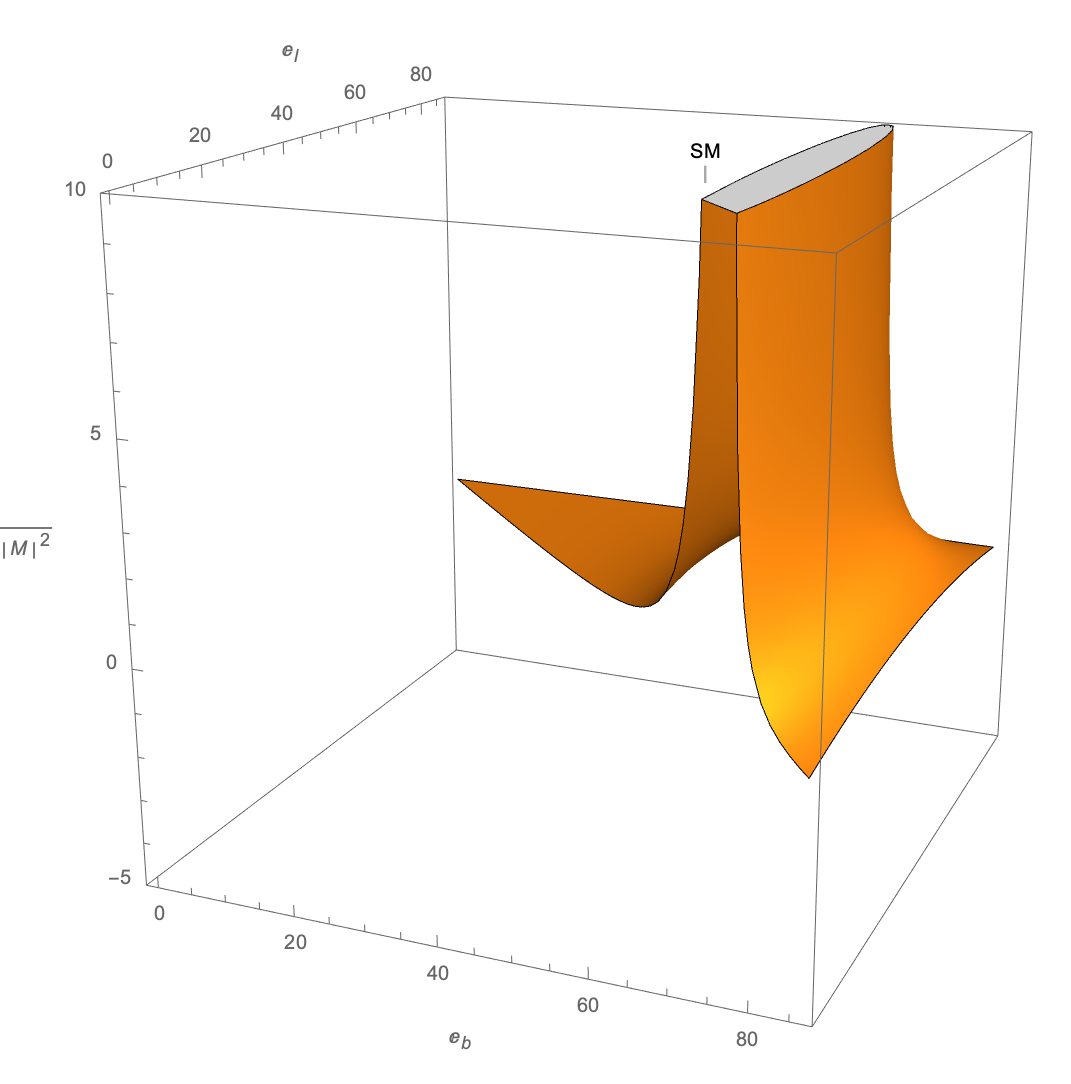
\includegraphics[width=0.4 \textwidth]{chapters/RelatedWorks/sectionBSM/figures/SM.png}
    \caption{The SM $\overline{ |\mathcal{M}|^2 } $ as a function on the $(E_1,E_3)$ plane. The SM $\overline{ |\mathcal{M}|^2 } $  shows a sharp peak with non-zero width at $E_3 = \frac{m^2_t - m^2_W}{2 m_t} = 67.8 $ GeV. The top total width is proportional to the integral of $\overline{ |\mathcal{M}|^2 } $ within a triangle region on the $(E_1,E_3)$ plane. }
    \label{fig:relatedWorks:bsm:smTopDecay:smM2}
\end{figure}







\noindent where one can plug in $m_t= 173.1 \text{ GeV}, m_W= 80.6 \text{ GeV}, g=0.64 $  and $\Gamma_W = 2.07$ and evaluate the numerical value of the integral:
\begin{equation}
         \Gamma = 0.154 \text{ GeV} .
\end{equation} 


\noindent This result from the tree-level QFT calculation with Feynman rule  $\Gamma = 0.154 \text{ GeV} $ agrees well with the one calculated with the narrow width approximation $\Gamma^{NWA} = 0.157 \text{ GeV} $ in Equation~\ref{eqn:relatedWorks:bsm:nwa}. The agreement is a good check for the above calculations concerning the Feynman rule, spinnor math and the integral.





 
\subsection{Beyond Standard Model with \PWpr}
\label{sec:relatedWorks:bsm:WPrime}

\subsubsection{Model Overview}
\PWpr is a hypothetical massive gauge boson that couples to the electroweak charge current in many BSMs. So far, many direct searches for \PWpr boson have been conducted in the CMS and ATLAS at the LHC, including searches in the $W'\to \tau \nu$  channel (tau plus MET) \cite{Sirunyan:2018lbg, Khachatryan:2015pua,Aaboud:2018vgh}, $W'\to l \nu$ channel (electron or muon plus MET) \cite{Sirunyan:2018mpc, Aaboud:2017efa}, $W'\to W Z$ channel\cite{Sirunyan:2018ivv, Aaboud:2017eta}, $W'\to q_1 q_2$ channel \cite{Sirunyan:2016iap, Aaboud:2017yvp}, and $W'\to t b$ channel \cite{Sirunyan:2017vkm, Aaboud:2018juj}. The direct searches for \PWpr are usually model-independent, where an excess of data with respect to the SM prediction is searched in the corresponding invariant mass spectrum. Then the limits of the \PWpr mass are set in the context of Sequential Standard Model (SSM), in which no specific assumption is made on the BSM gauge structures, and \PWpr coupling to fermions is the same as \PW coupling to fermion in the SM. So SSM is the most generic \PWpr BSM with the least extra assumption on top of SM. The ATLAS experiment has excluded an SSM \PWpr for masses below 3.7 TeV in the $\tau+MET$ channel. The CMS experiment has excluded an SSM \PWpr for masses below 5.2 TeV in the combination of electron and muon channels. The current PDG combined limit of the $m_{W'}$ is also 5.2 TeV in the context of SSM. In contrast to the direct search, interpreting the potential LUV in the \PWpr-mediated top decay is more model-dependent. This subsection presents an overview of the \PWpr BSMs and then focuses on the most relevant \PWpr models, the Nonuniversal G221 model.




One of the most common ways to model the new physics is to extend the structure of the SM gauge symmetry. The extension of the gauge symmetry consequently introduces new gauge bosons, such as \PWpr. Though there are many possible ways to extend the SM $SU(2)_L \times U(1)_Y $ to a larger symmetry group, such as the grand unification models with a SU(5) symmetry, one of the simplest and the most widely studied extension is $SU(2)_1 \times SU(2)_2 \times U(1)_X $. Models based on such gauge extension are commonly called G221 models \cite{Hsieh:2010zr}. Though having the same underline gauge structure, different G221 models can embed different fermion doublets in the $SU(2)_1$ and $SU(2)_2$ group, thus predicting different physics. Depending on the physical contents assigned to the $SU(2)_1 \times SU(2)_2 \times U(1)_X $ group, the G221 models are largely classified into three types: Left-Right \cite{PhysRevD.11.2558}, Ununified \cite{Chivukula:1994qw, GEORGI1990541} and Nonuniversal \cite{PhysRevLett.47.1788, MULLER1997192, PhysRevD.81.015006}.




\begin{itemize}
    \item Left-Right. The $SU(2)_1$ and $SU(2)_2$ in the left-right G221 describe the left-handed and right-handed fermion doublets, respectively. The fermion doublets involve both lepton and quarks. There are variations in which the right-handed fermion doublets are comprised of only leptons or quarks. The left-handed fermion doublets in the $SU(2)_1$ group are the same as those in the SM; the right-handed fermion doublet in the $SU(2)_2$ assumes the existence of right-handed neutrinos with masses beyond the TeV scale. In the low energy domain, the combination of the $SU(2)_2$ and the BSM $U(1)_X$ symmetry spontaneously breaks into the SM hypercharge symmetry $U(1)_Y$. Namely, the BSM breaking step is $SU(2)_2 \times U(1)_X  \to U(1)_Y$, which gives masses to the new gauge bosons like \PWpr. While the \PW couples to left-handed doublets like SM, \PWpr couples to the right-handed doublets. Besides, W' could have a suppressed coupling to the left-handed doublets via the W-W' mixing. 
    
    \item Ununified. The $SU(2)_1$ and $SU(2)_2$ in the ununified G221 describe the lepton doublets and quark doublets, respectively. The $U(1)_X$ is the same as the SM hypercharge symmetry,  $U(1)_X=U(1)_Y$. The name ``ununified" highlights that leptons and quarks have separate underline symmetries. The two separate quark and lepton symmetries break into a single symmetry, the SM $SU(2)_L$, in the low energy domain. Namely, the BSM breaking step is $SU(2)_1 \times SU(2)_2 \to SU(2)_L$, which gives masses to the new gauge bosons like \PWpr. The coupling of \PWpr is mainly to the quark currents, which leads to a potential enhancement in the quark-involved processes.

    \item Nonuniversal. The $SU(2)_1$ and $SU(2)_2$ in the nonuniversal G221, sometimes referred to as nonuniversal gauge interaction models (NUGIM), describe the fermion doublets in the first two generations and fermion doublets in the third generation, respectively. The $U(1)_X$ is the same as the SM hypercharge symmetry,  $U(1)_X=U(1)_Y$. The name ``nonuniversal" implies that the first two generations and the third generation are embedded into separate $SU(2)$ groups. The BSM breaking is the same as the ununified G221, $SU(2)_1 \times SU(2)_2 \to SU(2)_L$. There is a mixing angle $\theta_E$ between the $SU(2)_1$ and $SU(2)_2$ groups. Thus, \PWpr couplings to the third generation and the first two generations are scaled by $\cot \theta_E$ and $\tan \theta_E$ respectively, leading to potential nonuniversal effects in the weak processes.
\end{itemize}




Among the three types, the most relevant model is the Nonuniversal G221 model, which is intended to violate the universality in the weak sector. Now, we focus on the nonuniversal G221 model or NUGIM and evaluate our analysis's sensitivity to this model. The interaction Lagrangian in the NUGIM originates from the covariant derivatives for light (gen=1,2) and heavy (gen=3) fermions. Denoting the coupling constants in the $SU(2)_1 , SU(2)_2, U(1)_X$ as $g_1, g_2, g'$, the covariant derivatives are
\begin{equation}
\begin{split}
	D_\mu \psi_{gen=1,2} &= \big[ \partial_\mu -ig_1W^a_{1\mu} T^a P_L - ig'YB_\mu\big] \psi_{gen=1,2}  \\
    D_\mu \psi_{gen=3} &= \big[ \partial_\mu -ig_2W^a_{2\mu} T^a P_L - ig'YB_\mu\big] \psi_{gen=3} 
\end{split}
\label{eqn:relatedWorks:bsm:WPrime:derivative}
\end{equation}

\noindent Given the mixing angle $\theta_E$ between the $SU(2)_1$ and $SU(2)_2$ group, the underline coupling constants $g_1, g_2$ are related to the SM weak coupling constant $g$ by
\begin{equation}
	g_1=g/ \cos \theta_E, \quad g_2=g/ \sin \theta_E.
\end{equation}

\noindent And the SM $W^a$ triplet fields and new BSM triplet fields $W'^a$  are the mixing states of $W_1^a$ and $W_2^a$:
\begin{equation}
	W^a = \frac{g_1 W^a_1 + g_2 W_2^a}{\sqrt{g_1^2+g_2^2}} \quad W'^a = \frac{-g_1 W^a_1 + g_2 W_2^a}{\sqrt{g_1^2+g_2^2}}
\end{equation}

\noindent NUGIM employs two higgs doublets to generate mass for gauge bosons, including W and W'. Different from the standard 2HDM which is discussed in Section~\ref{sec:relatedWorks:bsm:chargedHiggs}, here the two higgs doublets are responsible for the first two generations and the third generation fermions. A large Higgs VEV ratio between the two doublets, $\tan \beta$, can explain the relative smallness of masses in the first two generations compared to the top quark, whereas it does not explain the hierarchy $m_t > m_b$. This is in contrast to the 2HDM Type-II models where large $\tan \beta$ can explain the hierarchy $m_b\ll m_t$, but not $m_u, m_c  \ll m_t$. Given the covariant derivatives in Equation~\ref{eqn:relatedWorks:bsm:WPrime:derivative} and the mixing angle $\theta_E$, the Feynman rule for \PWpr couplings \cite{Edelhauser:2014yra} to the light and heavy fermion currents are 
\begin{equation}
\begin{split}
	\bar{t} b W'^+ , \bar{\tau} \nu_\tau W+ \Longrightarrow -\frac{i g}{\sqrt{2}} \cot_E \gamma^\mu P_L \\
    \bar{u} d W'^+ , \bar{e} \nu_e W+ \Longrightarrow -\frac{i g}{\sqrt{2}} \tan_E \gamma^\mu P_L
\end{split}
\label{eqn:relatedWorks:bsm:WPrime:feynmanRule}
\end{equation}

\noindent and the Feynman rule for the propagator \PWpr takes a similar form to the SM W in Equation~\ref{eqn:relatedWorks:bsm:wPropagator}:
\begin{equation}
    \feynmandiagram [inline=(d.base), horizontal=d to b] {
        d -- [boson, edge label=\(W`^{\pm}\), momentum'=\(q\)] b ,
    }; =
    -i \frac{g^{\mu \nu} - q^\mu q^\nu/m^2_{W'}  }{q^2 - m^2_{W'} + i m_{W'} \Gamma_{W'} } .
\end{equation}


In Equation~\ref{eqn:relatedWorks:bsm:WPrime:feynmanRule}, the larger is the parameter $\cot_E$, the more enhancement to the third generation and more suppression to the first two generations there would be. So $\cot_E$ is the key parameter in the NUGIM to control the degree of ``nonuniversality". Also based on  Equation~\ref{eqn:relatedWorks:bsm:WPrime:feynmanRule}, the total width and the branching fraction of \PWpr can be calculated \cite{Edelhauser:2014yra}. If we denote the decay rate of SM W to electron and neutrino in Equation~\ref{eqn:relatedWorks:bsm:wWidth} as $\Gamma_l=\frac{g^2 m_W}{48 \pi}$, the partial widths of \PWpr to the first two generations and the third generation fermion are 
\begin{equation}
\begin{split}
	\text{hadronic: } \quad & \Gamma_{W'\to tb}  = 3  \cot_E^2  \frac{W'}{W}\Gamma_l  = 3  \cot_E^2  \frac{g^2 m_{W'}}{48 \pi}, \quad  \Gamma_{W'\to ud}  = 3  \tan_E^2  \frac{W'}{W}\Gamma_l  = 3  \tan_E^2  \frac{g^2 m_{W'}}{48 \pi} \\
	\text{leptonic: } \quad & \Gamma_{W'\to \tau \nu}  = \cot_E^2  \frac{W'}{W}\Gamma_l  = \cot_E^2  \frac{g^2 m_{W'}}{48 \pi},  \quad  \Gamma_{W'\to e \nu}  =\tan_E^2  \frac{W'}{W}\Gamma_l  =  \tan_E^2  \frac{g^2 m_{W'}}{48 \pi} 
\end{split}
\end{equation}

\noindent It is also allowed that \PWpr decays into SM Higgs and \PW boson, $W' \to h +W$, width of which is $ \Gamma_{W'\to h W}  = \frac{1}{4} \Gamma_{W'\to \tau \nu} $  in the limit of large $\tan \beta$ corresponding to the SM fermion hierarchy \cite{KIM2012367}. Thus the total width of \PWpr sums up the hadronic, leptonic and Higgs emitting width;
\begin{equation}
	\Gamma_{W'} = \frac{g^2 m_{W'}}{48 \pi} \big [ (3+1+\frac{1}{4}) \cot^2_E + (6+2)\tan_E^2 \big] .
\end{equation}

\noindent where the width is proportional to the $ \cot^2_E $ or $ 1/\cot^2_E$ when $\cot^2_E \gg 1$ or $1 \gg \cot^2_E > 0$.  So NUGIM has a inbuilt upper and lower boundaries for $\cot_E$, constrained by the width of \PWpr. The parameter space beyond this boundaries predicts a \PWpr with too wide width to be physical.  Take a conservatively large width as an example. If the width is smaller than $50\%$ of the \PWpr mass, then 
\begin{equation}
    0.21 < \cot_E < 6.48.
\end{equation}


\begin{figure}[ht]
    \centering
    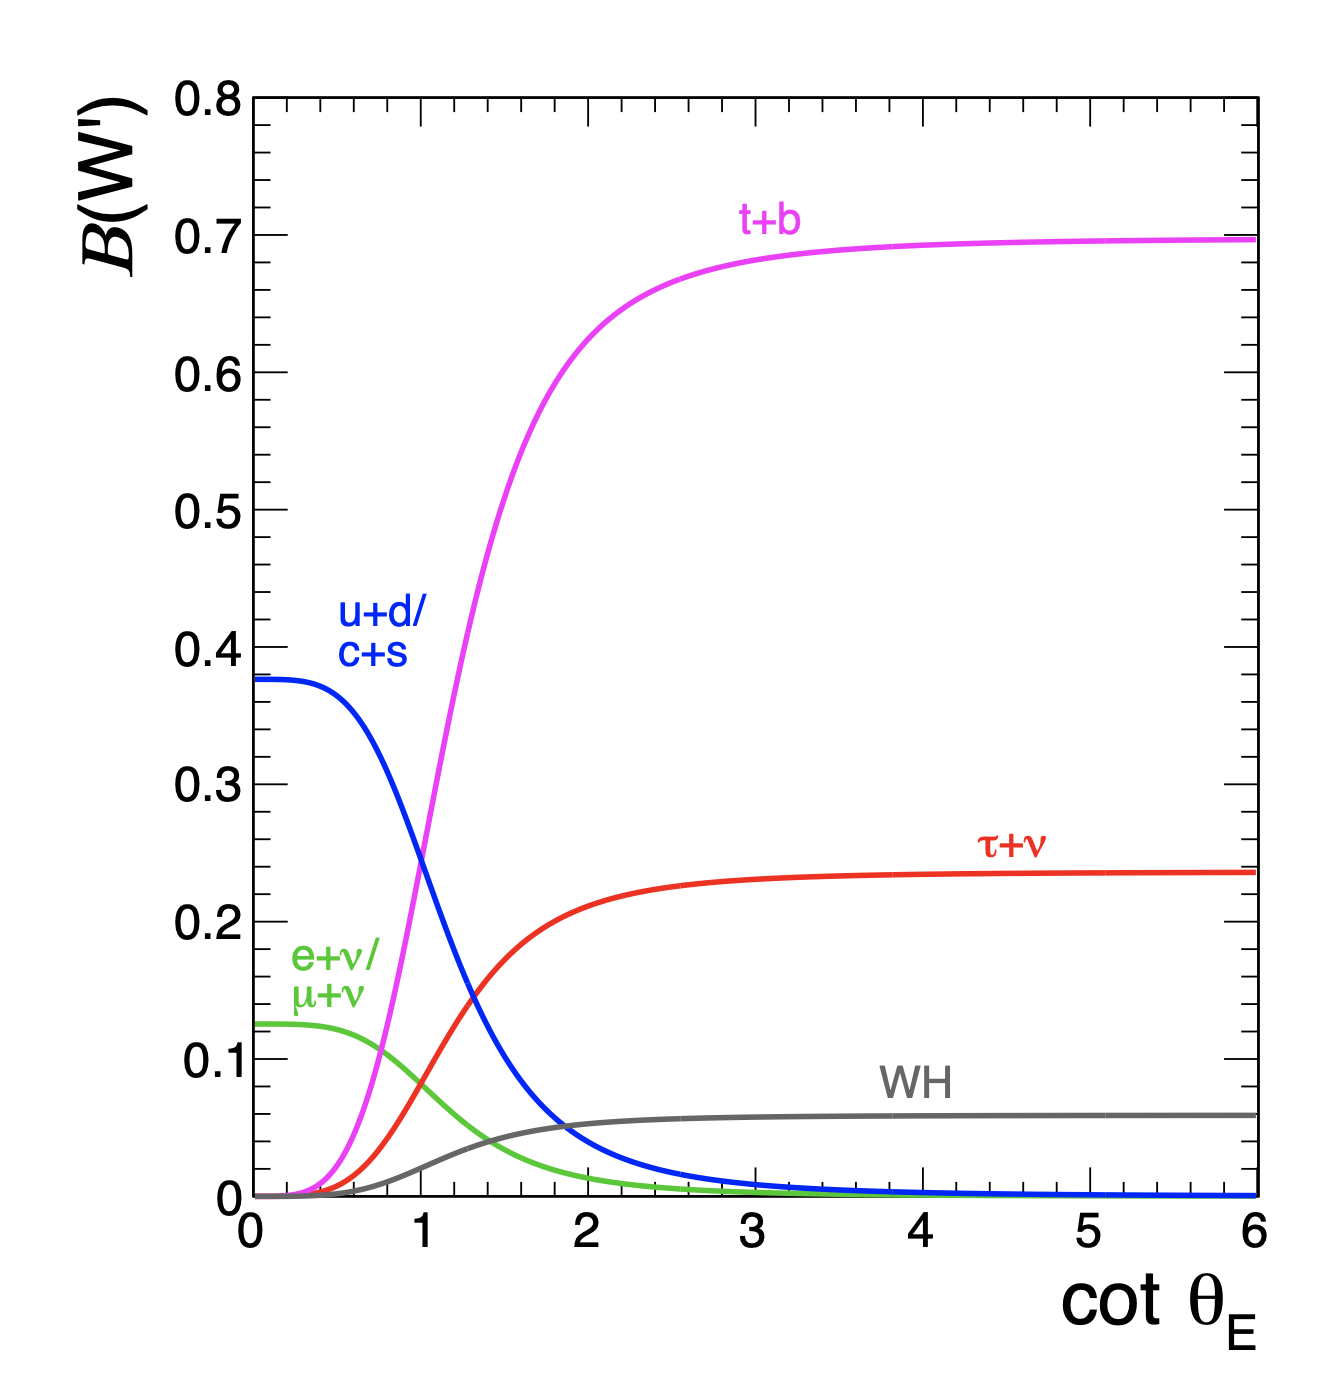
\includegraphics[width=0.4\textwidth]{chapters/RelatedWorks/sectionBSM/figures/WPDecayBr.png}
    \caption{The branching fraction of W' in NUGIM as a function of $\cot_E$ \cite{Sirunyan:2018lbg}. $\cot_E$ is the parameter controlling the degree of nonuniversality.}
    \label{fig:relatedWorks:bsm:WPrime:braching}
\end{figure}



\noindent The branching fraction of W' is shown in Figure~\ref{fig:relatedWorks:bsm:WPrime:braching}. When $\cot_E > 2$, W' decays dominantly to the third family fermions and the branching ratio to the first two generation is neglectable. The situation is reversed when $\cot_E<0.5$ .


\subsubsection{Enhancement of Tauonic Top Width}

The total $\overline{ |\mathcal{M}|^2 }$ in the NUGIM not only has the contributions from the SM W boson in Section~\ref{sec:relatedWorks:bsm:smTopDecay}, but also includes diagrams for W' $\overline{ |\mathcal{M}|^2 } _{W'} $  and the interference between the W and W' $\overline{ |\mathcal{M}|^2 } _{int} $ . Namely,
\begin{equation}
	\overline{ |\mathcal{M}|^2 }  = \overline{ |\mathcal{M}|^2 } _{W} +  \overline{ |\mathcal{M}|^2 } _{W'} +  \overline{ |\mathcal{M}|^2 } _{int} .
\end{equation}

\noindent where the SM part $\overline{ |\mathcal{M}|^2 } _{W} $  has been calculated in Equation~\ref{eqn:relatedWorks:bsm:smTopDecay:smTopDecay:m2}, while $\overline{ |\mathcal{M}|^2 } _{W'} +  \overline{ |\mathcal{M}|^2 } _{int}$ is the new BSM contribution we need to evaluate now. This BSM contribution enhances the tau channel in the top decay. Eventually, the ratio of this BSM contribution over the SM contribution will be estimated and compared with our experimental precision. Now consider $\cot_E > 2$ where the BSM branching fraction to first and second generation of leptons are neglectable. With Feynman rule, the matrix element of top's tauonic decay mediated by W', similar to Equation~\ref{eqn:relatedWorks:bsm:smTopDecay:smTopDecay:m}, is spelt as the \PWpr propagator sandwiched by two fermion currents and scaled by the coupling constant squared:
\begin{equation}
\begin{split}
	i \mathcal{M}_{W'}  & =  (\frac{g \cot_E}{\sqrt{2}})^2 \cdot 
	\big[ \bar{u}_3 \gamma_\mu P_L u_a \big] 
	\frac{g^{\mu \nu} - q^\mu q^\nu/M^2_{W'}}{q^2-m^2_{W'} + i m_{W'} \Gamma_{W'}} 
	\big[ \bar{u}_2 \gamma_\nu P_L v_1 \big] .
\end{split}
\end{equation}

\noindent The calculation of the average amplitude squared  $\overline{ |\mathcal{M}|^2 } _{W'} $ and $\overline{ |\mathcal{M}|^2 } _{int}$ has the same mathematical process as that in Section~\ref{sec:relatedWorks:bsm:smTopDecay}. First sum the spins; then evaluate the traces of gamma matrices. The result of such calculation reads as
\begin{equation}
	\overline{ |\mathcal{M}|^2 }_{W'} =  g^4 \cot_E^4 \frac{2  (  k_2 \cdot k_3) (  k_1 \cdot p_a) }{ (  q^2-m^2_{W'})^2 +  m^2_{W'} \Gamma^2_{W'} }  
\end{equation}

\noindent and
\begin{equation}
\begin{split}
    \overline{ |\mathcal{M}|^2 } _{int} = &   2 \overline{ Re[\mathcal{M}^*_W \mathcal{M}_{W'}] }  \\
    =& 2 g ^4\cot^2_E  \cdot  [2  (  k_2 \cdot k_3) (  k_1 \cdot p_a) ] \cdot \\
    &\frac 
    {( q^2-m^2_{W}) ( q^2-m^2_{W'}) + m^2_{W}  m^2_{W'}  \Gamma^2_{W} \Gamma^2_{W'} }
    { \big[ ( q^2-m^2_{W})^2 +  m^2_{W} \Gamma^2_{W} \big] \big[ (  q^2-m^2_{W'})^2 +  m^2_{W'} \Gamma^2_{W'} \big] }   
    ,
\end{split}
\end{equation}

\noindent where the inner products $(  k_2 \cdot k_3)$ and $ (  k_1 \cdot p_a) $ can be represented in terms of $(E_1,E_3)$ using Equation~\ref{eqn:relatedWorks:bsm:innerProduct}. Then $\overline{ |\mathcal{M}|^2 } _{W'} $ and $\overline{ |\mathcal{M}|^2 } _{int}$ become 2D functions on the $(E_1,E_3)$ plane with two model parameters $(\cot_E, m_{W'})$.  Figure~\ref{fig:relatedWorks:bsm:WPrime:m2} shows a visualization of the $\overline{ |\mathcal{M}|^2 } _{W'} $ and $\overline{ |\mathcal{M}|^2 } _{int}$ on the $(E_1,E_3)$ plane, overlapped with the SM $\overline{ |\mathcal{M}|^2 } _{W}$ from Section~\ref{sec:relatedWorks:bsm:smTopDecay}. The $\overline{ |\mathcal{M}|^2 } _{W}$, $\overline{ |\mathcal{M}|^2 } _{W'} $ and $\overline{ |\mathcal{M}|^2 } _{int}$ are shown as orange, blue and green surface, respectively. The upper left plot in Figure~\ref{fig:relatedWorks:bsm:WPrime:m2} shows the scenario of
$\cot_E=1, m_{W'}=140 \text{ GeV}$, where W' is light enough to be on-shell from the top decay and  $\overline{ |\mathcal{M}|^2 } _{W'} $ has a clear peak at $E_3 = (m^2_t - m^2_{W'})/2 m_t $. Due to this on-shell peak,  $\overline{ |\mathcal{M}|^2 } _{W'} $ is much larger than the interference term  $\overline{ |\mathcal{M}|^2 } _{int}$  and is the dominating BSM contribution. As $m_{W'}$ increases, the on-shell W' peak moves to left towards smaller $E_3$ and eventually disappear in the triangle area when $m_{W'} > m_{t}$. Upper right plot in Figure~\ref{fig:relatedWorks:bsm:WPrime:m2} shows the scenario of $\cot_E=1, m_{W'}=300 \text{ GeV}$, where the blue peak is out side the triangle area and the leading BSM contribution is from the interference. The lower plot in Figure~\ref{fig:relatedWorks:bsm:WPrime:m2} increases the $\cot_E$  with $\cot_E=4, m_{W'}=300 \text{ GeV}$, where W' width is wider and the interference becomes stronger. 





\begin{figure}[ht]
    \centering
    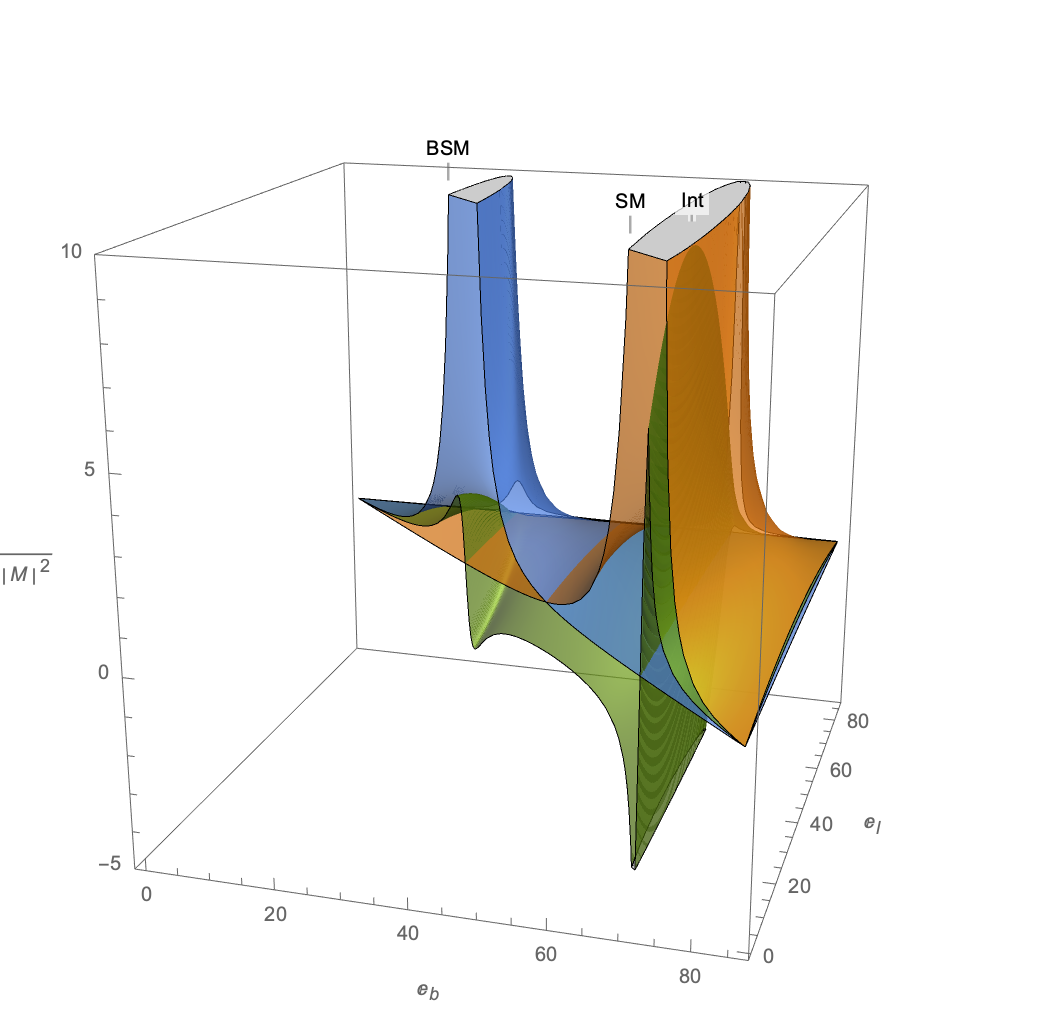
\includegraphics[width=0.49\textwidth]{chapters/RelatedWorks/sectionBSM/figures/WPrime_140_1.png}
    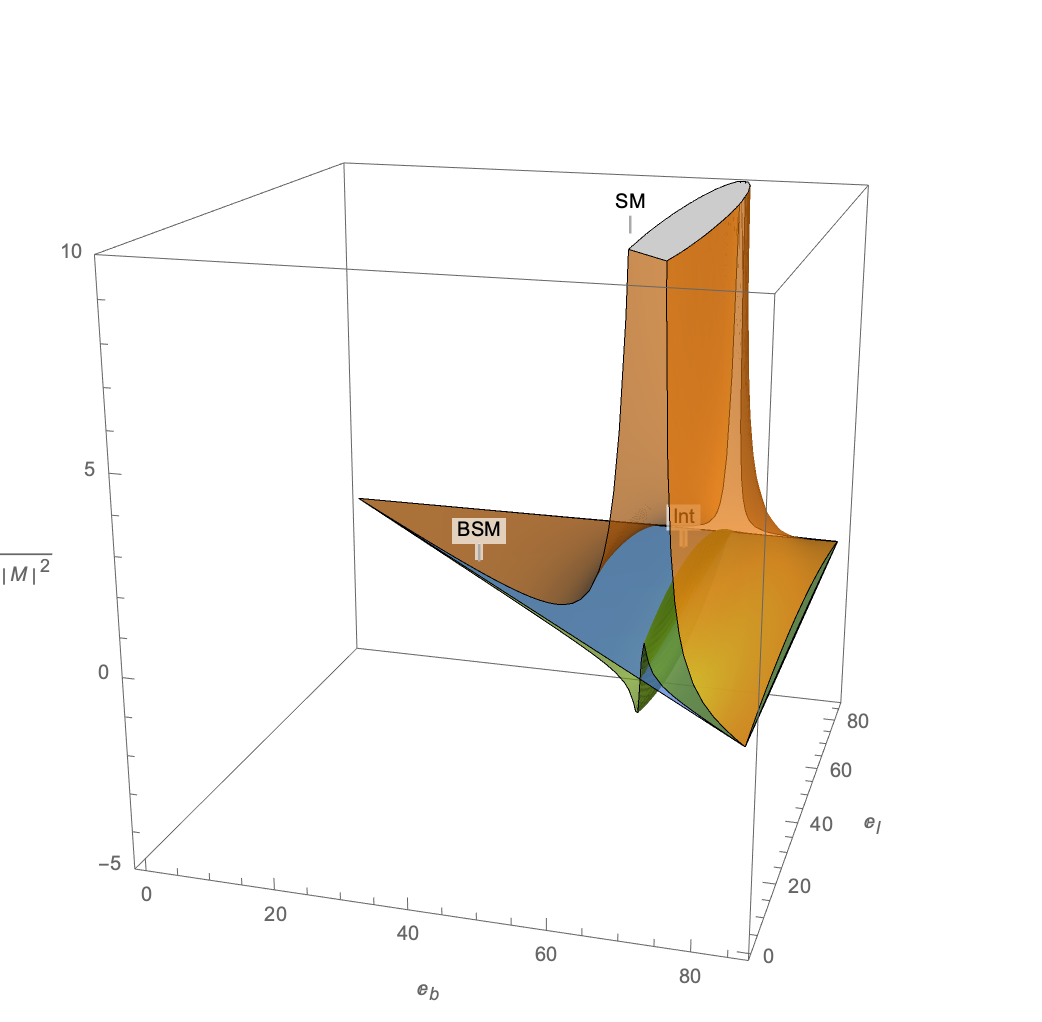
\includegraphics[width=0.49\textwidth]{chapters/RelatedWorks/sectionBSM/figures/WPrime_300_1.png}
    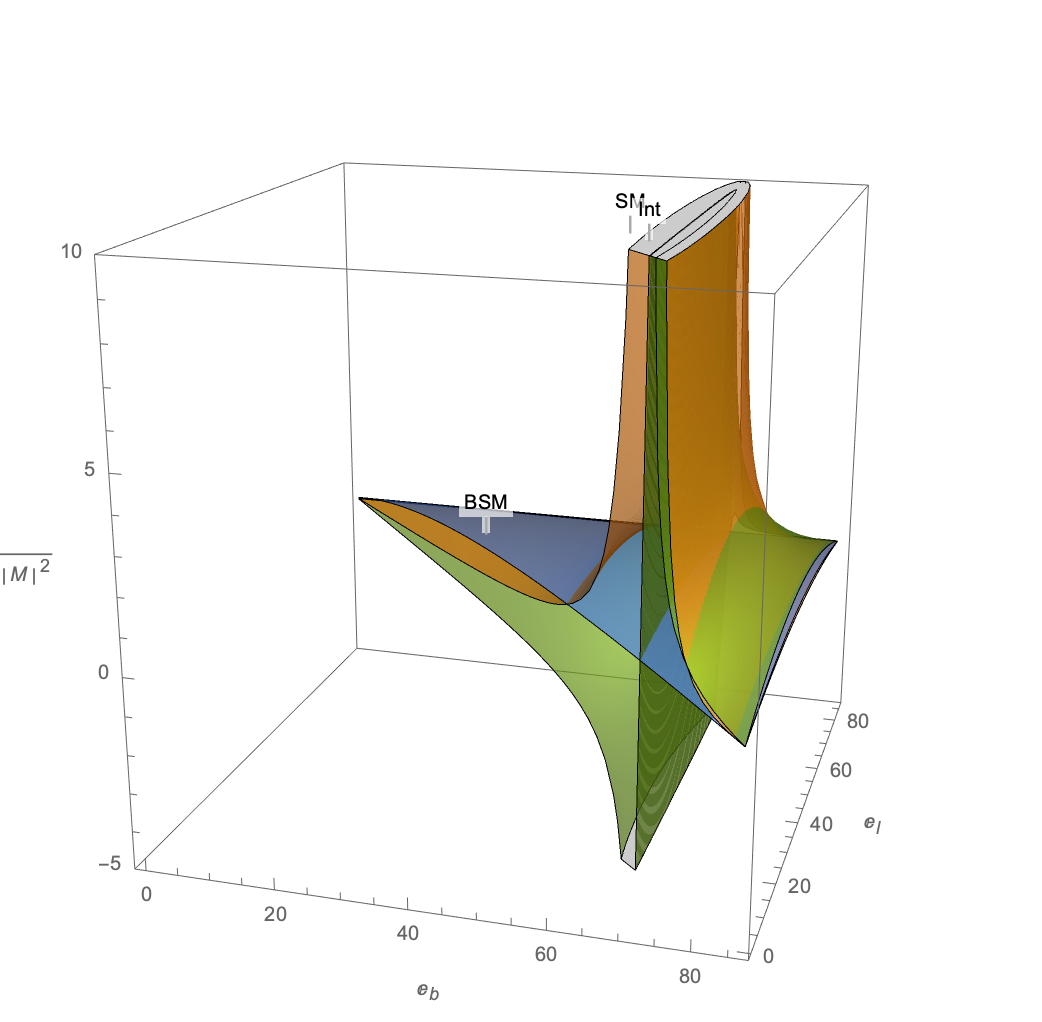
\includegraphics[width=0.49\textwidth]{chapters/RelatedWorks/sectionBSM/figures/WPrime_300_4.png}
    \caption{ $\overline{ |\mathcal{M}|^2 } _{W}$, $\overline{ |\mathcal{M}|^2 } _{W'} $ and $\overline{ |\mathcal{M}|^2 } _{int}$ on the $(E_1,E_3)$ plane. These three functions correspond to the orange, blue and green surface, respectively. Changing the two model parameters $(\cot_E, m_{W'})$ leads to different scenarios of $\overline{ |\mathcal{M}|^2 } _{W}$, $\overline{ |\mathcal{M}|^2 } _{W'} $ and $\overline{ |\mathcal{M}|^2 } _{int}$. Upper left, upper right and lower plots illustrate  $(\cot_E=1, m_{W'}=140  \text{ GeV} )$, $(\cot_E=1, m_{W'}=300  \text{ GeV} )$ , and $(\cot_E=4, m_{W'}=300  \text{ GeV} )$ cases. }
    \label{fig:relatedWorks:bsm:WPrime:m2}
\end{figure}



Upon integrating  $\overline{ |\mathcal{M}|^2 } _{W'} +  \overline{ |\mathcal{M}|^2 } _{int}$ on the $(E_1,E_3)$ plane using Equation~\ref{eqn:relatedWorks:bsm:decayWidth}, one gets the BSM width of the taunic top decay $\Gamma^{BSM}$. 
\begin{equation}
	\Gamma^{BSM} = \frac{1}{64 \pi^3 m_t} \int_{0}^{m_t/2} dE_3 \int_{m_t/2-E_3}^{m_t/2} dE_1  \bigg\{ \overline{ |\mathcal{M}|^2 } _{W'} +  \overline{ |\mathcal{M}|^2}_{int}  \bigg \},
\end{equation}


\noindent Then the relative tau enhancement from the BSM with respect to SM can be obtained by $\Gamma^{BSM}/ \Gamma^{SM}$, where $\Gamma^{SM}=154$ MeV. For example, when $\cot_E=6$  and $m_{W'}=1$ TeV, $\overline{ |\mathcal{M}|^2 } _{W'} +  \overline{ |\mathcal{M}|^2 } _{int}$ integral yields $\Gamma^{BSM} = 0.86 $ MeV and tau enhancement is
\begin{equation}
	\frac{ \Gamma_{t\to b \tau \nu_\tau}^{BSM} }{ \Gamma_{t\to b \tau \nu_\tau}^{SM} } \sim 0.55 \%, \quad (\cot_E=6, m_{W'}=1 \text{ TeV}).
\end{equation}

\noindent In addition to this example $(\cot_E, m_{W'})$, the tau enhancement $ \Gamma_{t\to b \tau \nu_\tau}^{BSM} / \Gamma_{t\to b \tau \nu_\tau}^{SM} $ can be calculated in the model parameters space $(\cot_E, m_{W'})$ , shown as Figure~\ref{fig:relatedWorks:bsm:WPrime:tauEnhancement}. The relative tau enhancement decrease as $m_{W'}$ increases and $\cot_E$ approaches to 1. For $\cot_E=4,6,10$, the $\Gamma_{t\to b \tau \nu_\tau}^{BSM}/  \Gamma_{t\to b \tau \nu_\tau}^{SM} $ as a 1D function of W' mass, decomposed into $\overline{ |\mathcal{M}|^2 } _{W'} $ and $\overline{ |\mathcal{M}|^2 } _{int}$  parts, is shown in Figure~\ref{fig:relatedWorks:bsm:WPrime:tauEnhancement1d}. In Figure~\ref{fig:relatedWorks:bsm:WPrime:tauEnhancement}, the contours correspond per-mil and percent level enhancement are shown as white dash lines, the upper boundary of $\cot_E$ is shown as the black line. Our analysis confirms lepton universality and no tau enhancement with a $2\%$ relative uncertainty, which translate to exclusion of $ \Gamma_{t\to b \tau \nu_\tau}^{BSM} / \Gamma_{t\to b \tau \nu_\tau}^{SM} >  2\%$ with 0.68 confidence integral, shown as the left side of the green contour. $ \Gamma_{t\to b \tau \nu_\tau}^{BSM} / \Gamma_{t\to b \tau \nu_\tau}^{SM} >  4\%$ is shown as the left side of the blue contour. For $m_{W'}>600$ GeV, our exclusion region is beyond the the model's upper boundary of $\cot_E$ and not as competitive as the direct searches, shown in Figure~\ref{fig:relatedWorks:bsm:WPrime:directSearch}.




\begin{figure}
    \centering
    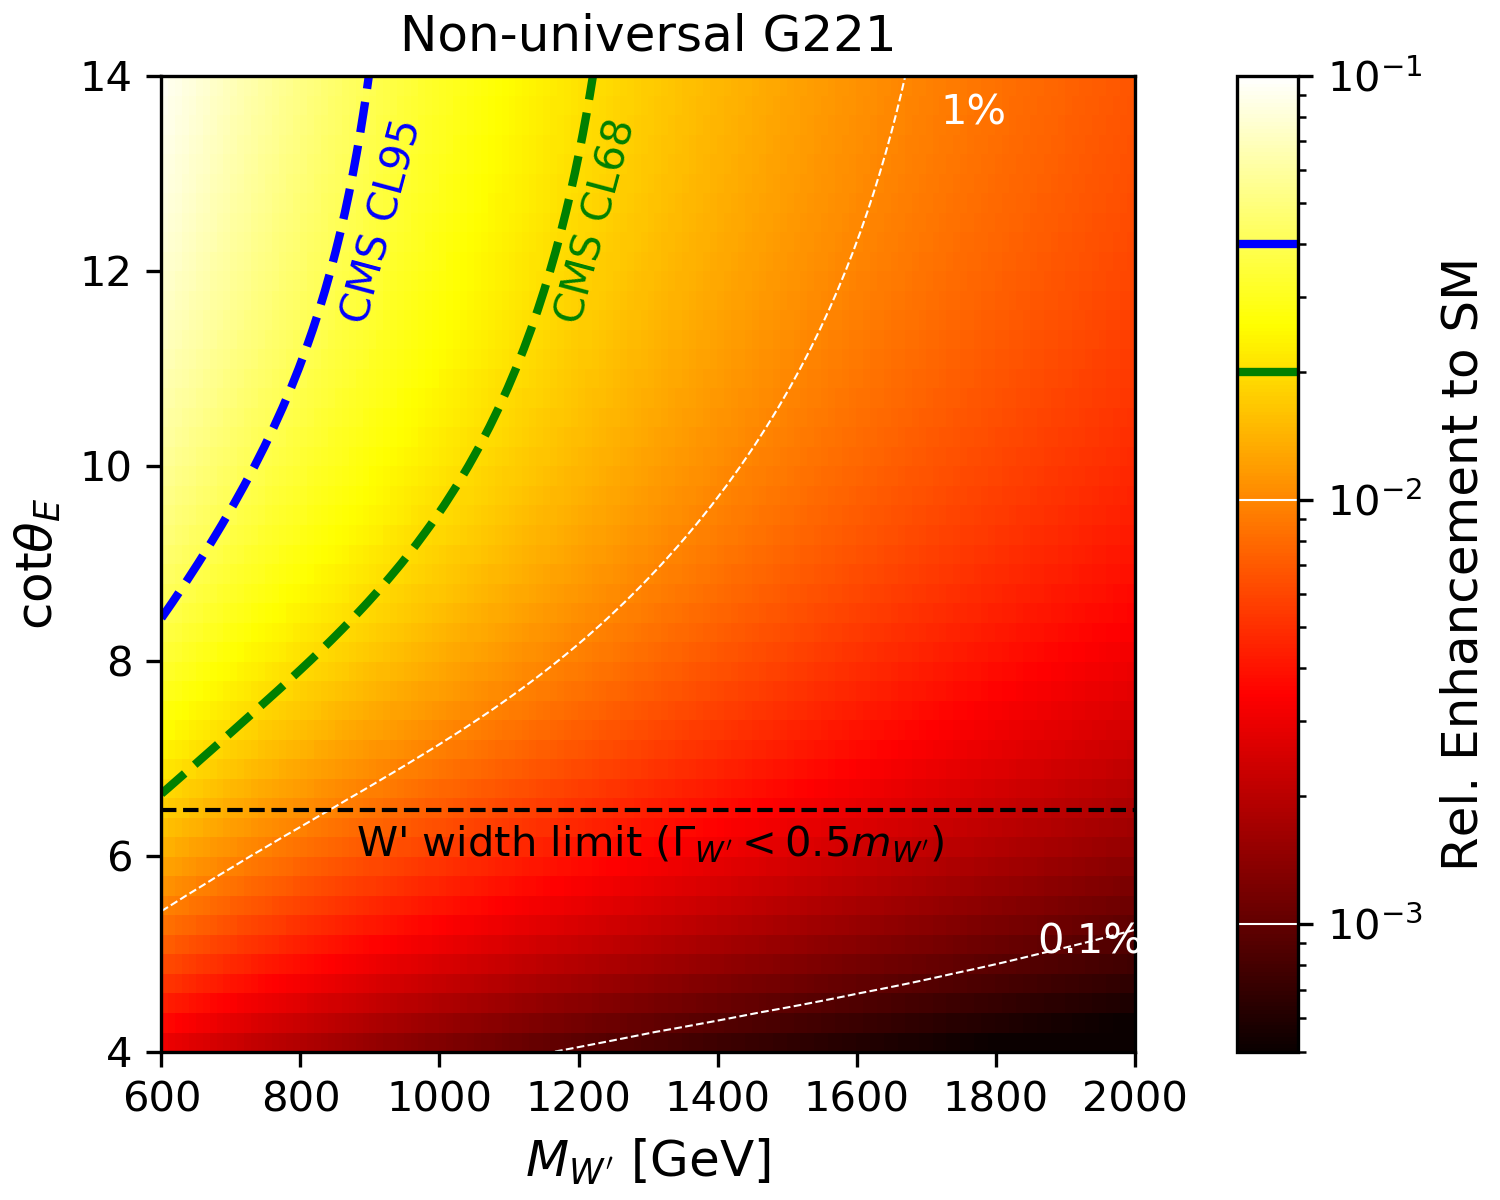
\includegraphics[width=0.6\textwidth]{chapters/RelatedWorks/sectionBSM/figures/RelEnhance.png} 
    \caption{The relative tau enhancement $ \Gamma_{t\to b \tau \nu_\tau}^{BSM} / \Gamma_{t\to b \tau \nu_\tau}^{SM} $ in the NUGIM parameter space $(\cot_E, m_{W'})$. $\Gamma_{t\to b \tau \nu_\tau}^{BSM} $ is calculated from integrating $\overline{ |\mathcal{M}|^2 } _{W'} +  \overline{ |\mathcal{M}|^2 } _{int}$, while $\Gamma_{t\to b \tau \nu_\tau}^{SM}=154$ MeV in Section~\ref{sec:relatedWorks:bsm:smTopDecay}.  Our analysis confirm LU with 2\% uncertainty on the $B(W\to \tau \nu)$, excluding the $ \Gamma_{t\to b \tau \nu_\tau}^{BSM} / \Gamma_{t\to b \tau \nu_\tau}^{SM} <2\% $ with 0.68 confidence interval, shown as the left side of the blue contour.}
    \label{fig:relatedWorks:bsm:WPrime:tauEnhancement}
\end{figure}


\begin{figure}
    \centering
    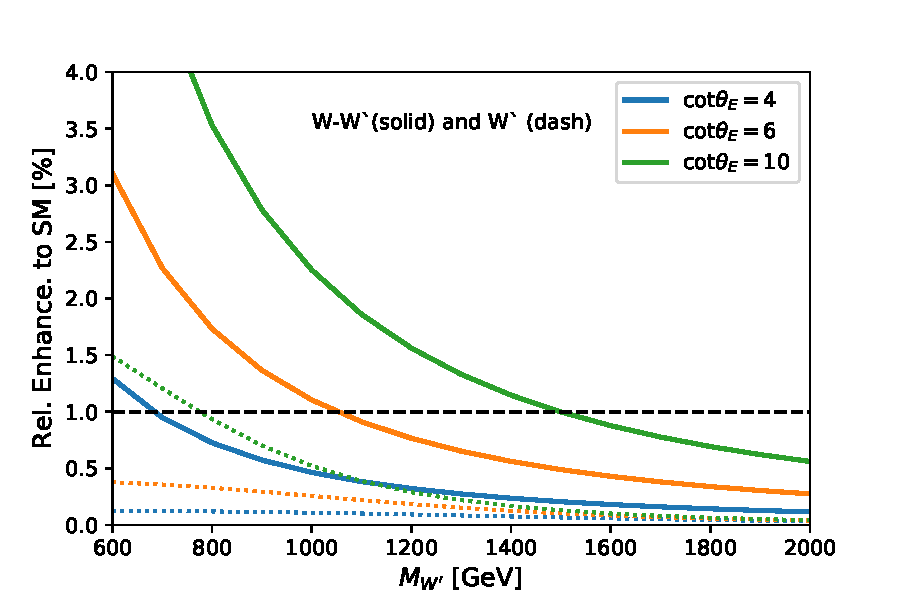
\includegraphics[width=0.6\textwidth]{chapters/RelatedWorks/sectionBSM/figures/RelEnhance1D.pdf} 
    \caption{For $\cot_E=4,6,10$, the $\Gamma_{t\to b \tau \nu_\tau}^{BSM}/  \Gamma_{t\to b \tau \nu_\tau}^{SM} $ as 1D function of W' mass is composited into $\overline{ |\mathcal{M}|^2 } _{W'} $ and $\overline{ |\mathcal{M}|^2 } _{int}$  parts, shown as dash and solid line respectively. For \PWpr heavier than top quark, the leading BSM contribution is from the W-W' interference term. }
    \label{fig:relatedWorks:bsm:WPrime:tauEnhancement1d}
\end{figure}



\begin{figure}
    \centering
    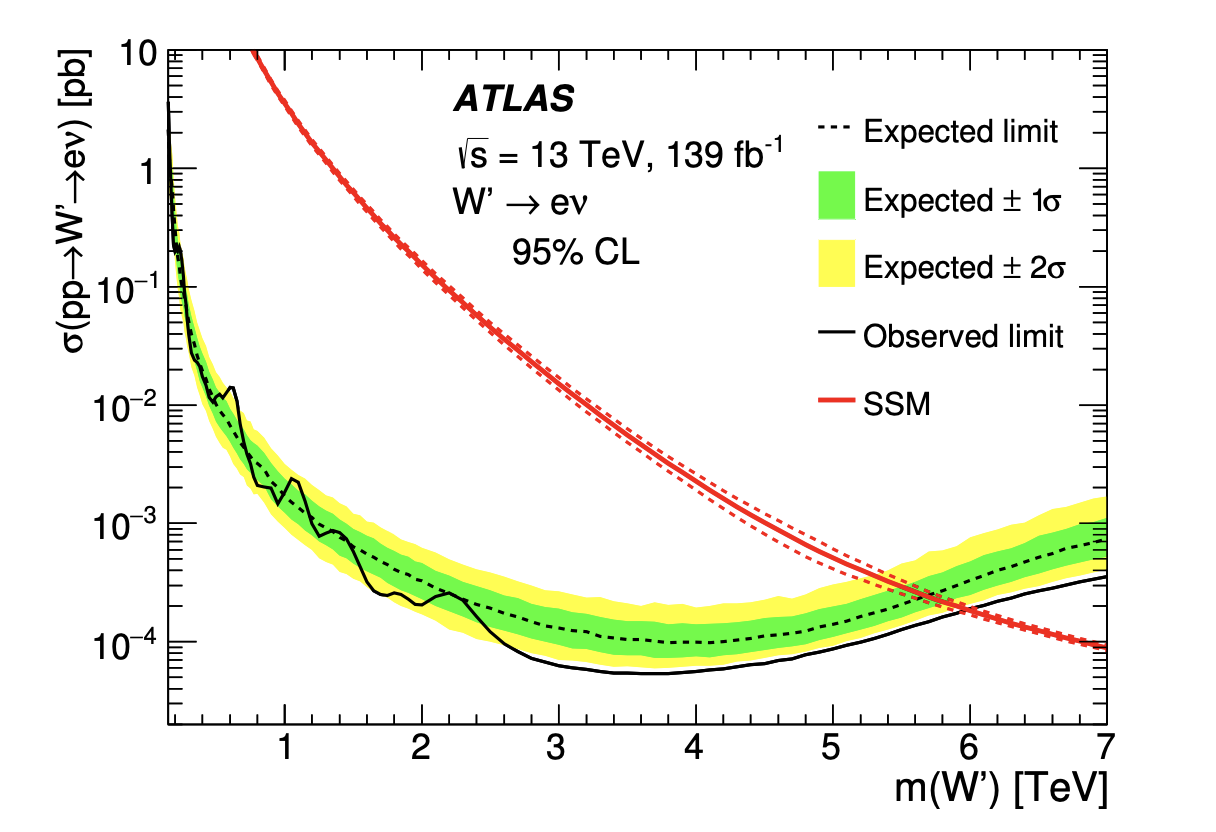
\includegraphics[width=0.49\textwidth]{chapters/RelatedWorks/sectionBSM/figures/WPrime_search0.png} 
    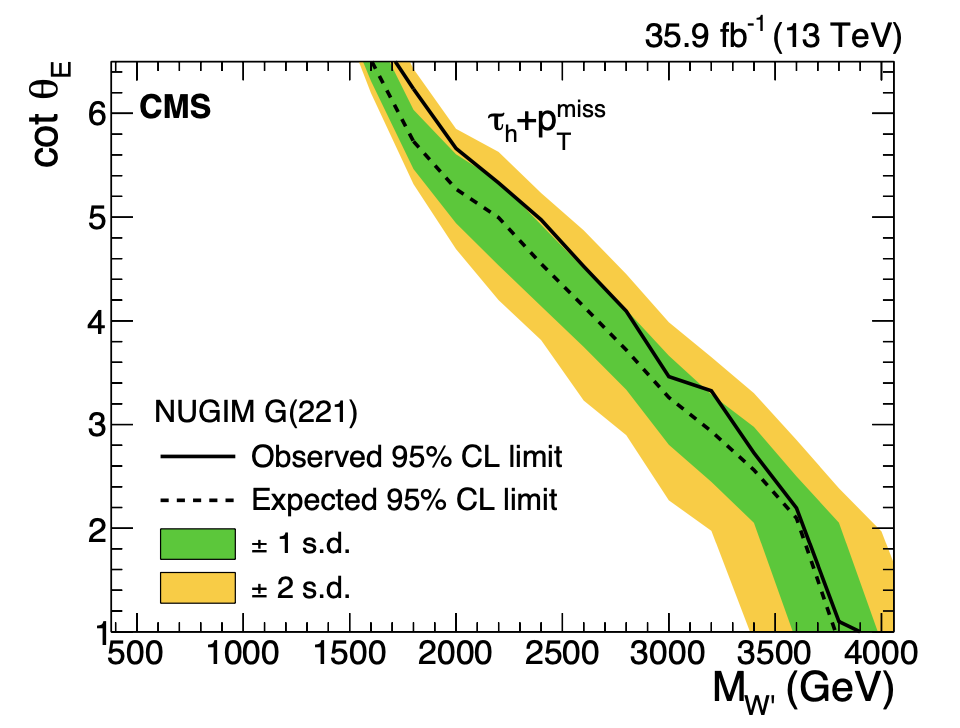
\includegraphics[width=0.49\textwidth]{chapters/RelatedWorks/sectionBSM/figures/WPrime_search.png} 
    \caption{Direct Search of W' on the Atlas and CMS.}
    \label{fig:relatedWorks:bsm:WPrime:directSearch}
\end{figure}






\FloatBarrier



% \begin{equation}
% 	\frac{ \Gamma_{t\to b \tau \nu_\tau}^{BSM} }{ \Gamma_{t\to b \tau \nu_\tau}^{SM} } \sim 7\times 10^{-5}
% \end{equation}
% Due to the large
% W' contribution to the measurement could be inbeded in the measurement. it could explain potential deviation form sm prediction.
% The decay of to
% \begin{equation}
% 	\frac{W'^{+}_{\mu}}{\sqrt{2}} \bigg[   \bar{u}_i (C^R_{q,ij} P_R + C^L_{q,ij} P_L) \gamma^\mu d_j   + \bar{\nu}_i (C^R_{l,ij} P_R + C^L_{l,ij} P_L) \gamma^\mu e_j \bigg]
% \end{equation}


% There are many models predicts w'. Other than grand unification models with SU(5) sysmmetry. Most popular models performs a minimum extension from the SM SU(2) sysmetry to $SU(2)_1 \times SU(2)_2$. At tree level, W' mixes with W. which is sensitive by the ew mixing angle or WZ mass ratio. So the experiment put a constraint on the the W-W' mxing to be small. In all gauge extension, W' would also couple to WZ via TGC and QGC, and couple to HW via higgs-gauge coupling. 

% In "left-right symmetric" model, The two SU(2) are for left and right doublet. the W couples to left-handed doublet while w' couples to the right handed doublet. W' could have a suppressed coupling to the left via the W-W' mixing. The sequential standard model assumes, right handed nuetrino are light and stable, W-W' mixing is zero. W' does not couple to left-handed fermions, the W' coupling to the right handed doublets is the same as W coupling to left fermion. 

% "un-unified model" , the two SU(2) are for lepton and quark doublet. During the SSB, four weak bosons are produced, the lighter W,Z behaves like SM and the W',Z' couples mainly to quarks.
% "topflavor model", the two SU(2) are for first second and third family of fermion doublet. This will cause a violation of lepton universality in the W sector. This thesis will gives a tight bound W' mass in this model.



% the most recent limit on w' is 5.2 TeV on the LHC 

% e,mu,tau,considering right nu decay to hadrons,  tb, WZ, WH

% 0v2b, Gf, KL-ks mixing, p vialation of polorized muon decay. 



\subsection{Beyond Standard Model with $H^+$}
\label{sec:relatedWorks:bsm:chargedHiggs}

\subsubsection{Model Overview}
The charged Higgs boson $H^+$ is a hypothetical particle in the BSM with an extended scalar field structure. In the SM, the scalar sector has the simplest possible structure, one SU(2) doublet. On the contrary, the fermion structure with three mixing families is not simple. It is possible that the scalar structure can have some more complex form. Two Higgs Doublet Model (2HDM) provides the next simplest structure for the SM scalar sector. It assumes one more scalar doublet in addition to that in the SM. The two scalar doublets are responsible for the mass of upper and lower fermions separately. There are three major motivations to 2HDM \cite{BRANCO20121}: generate mass in the Minimal Supersymmetric Standard Model (MSSM) \cite{HABER198575}, explain the strong CP in the QCD \cite{KIM19871, PhysRevLett.38.1440}, and adding extra CP-violation source for the baryon asymmetry \cite{Trodden:1998qg, TUROK1991471, Joyce:1994zt}. 

% (From Review \cite{BRANCO20121}) The first and the best-known motivation is supersymmetry \cite{HABER198575}. In the supersymmetric theories, the scalars belong to chiral multiplets and their complex conjugates belong to multiplets of the opposite chirality; since multiplets of different chiralities cannot couple together in the Lagrangian, a single Higgs doublet cannot give mass simultaneously to the upper-type and down-type quarks. Moreover, since scalars sit in chiral multiplets together with the chiral spin-$\frac{1}{2}$ fields, the cancellation of anomalies also requires an additional doublet. The second motivation for 2HDMs comes from axion models \cite{KIM19871}. Peccei and Quinn \cite{PhysRevLett.38.1440} noted that a possible CP-violating term in the QCD Lagrangian, which is phenomenologically known to be very small, can be rotated away if the Lagrangian contains a global symmetry. However, imposing this symmetry is only possible if there are two Higgs doublets. While the simplest versions of the Peccei–Quinn model (in which all the New Physics was at the TeV scale) are experimentally ruled out, there are variations with singlets at a higher energy scale that are acceptable, and the effective low-energy theory for those models still requires two Higgs doublets \cite{KIM19871}. The third motivation for 2HDMs is that the CV violation in the SM electroweak sector is not enough \cite{Trodden:1998qg} to generate a baryon asymmetry of the Universe of sufficient size. Two-Higgs-doublet models can do so due to the flexibility of their scalar mass spectrum \cite{Trodden:1998qg} and the existence of additional sources of CP violation. There have been many works on baryogenesis in the 2HDM \cite{TUROK1991471, Joyce:1994zt}. 

The direct searches for $H^+$ have been conducted in two parts of the phase space, $m_{H^+} < m_t$  and $m_{H^+} > m_t$ \cite{pdg2020}. For $m_{H^+} < m_t$, LEP \cite{Abbiendi:2013hk}, CMS \cite{Khachatryan:2015qxa} and ATLAS \cite{Aad:2014kga} have exclude $H^+$ with mass below 80 GeV, 155 GeV, and 140 GeV with 95\% confidence level respectively. For $m_{H^+} > m_t$, ATLAS has provide a $\tan\beta$-dependant exclusion of $m_{H^+}$ \cite{Aaboud:2018gjj}, more explicitly $m_{H^+}>181,129,390,894,1017,1103$ GeV at $\tan\beta=10,20,30,40,50,60$. CMS has also updated its result in the $m_{H^+} > m_t$ search using 13 TeV data [ref]. Here in this section, similar to NUGIM $W'$ model, we explore the effect of 2HDM $H^+$ in the top decay and evaluate the corresponding ``tau enhancement" with respect to SM.






In 2HDMs, there are two complex scalar doublets with eight fields:
\begin{equation}
	\Phi_1 = \begin{bmatrix} \phi_1^+ \\ \frac{\nu_1}{\sqrt{2}} + \frac{\rho_1+i\eta_1}{\sqrt{2}}  \end{bmatrix} , 
    \Phi_2 = \begin{bmatrix} \phi_2^+ \\ \frac{\nu_2}{\sqrt{2}} + \frac{\rho_2+i\eta_2}{\sqrt{2}}  \end{bmatrix}
\end{equation}

\noindent where the ratio of the VEV of the two doublets are
\begin{equation}
\tan \beta = \frac{\nu_2}{\nu_1},
\end{equation}

\noindent and $\tan \beta$  is an important parameter in the model. The potential for the two scalar doublets reads as
\begin{equation}
\begin{split}
V=& m_{11}^2 \Phi_1^\dagger \Phi_1 + m_{22}^2 \Phi_2^\dagger \Phi_2 - m_{12}^2 ( \Phi_1^\dagger \Phi_2+\Phi_2^\dagger \Phi_1) \\
&  +\frac{\lambda_1}{2}(\Phi_1^\dagger \Phi_1)^2 +\frac{\lambda_2}{2}(\Phi_2^\dagger \Phi_2)^2
+\lambda_3 \Phi_1^\dagger \Phi_1 \Phi_2^\dagger \Phi_2 +\lambda_4 \Phi_1^\dagger \Phi_2 \Phi_2^\dagger \Phi_1
+\frac{\lambda_5}{2}[ (\Phi_1^\dagger \Phi_2)^2 + (\Phi_2^\dagger \Phi_1)^2 ]
\end{split}
\end{equation}

\noindent which is minimized when we choose the vacuum expectation value $\Phi_1= [0,v_1/\sqrt{2}]^T$ and $\Phi_2= [0,v_2/\sqrt{2}]^T$.



\noindent Out of the eight fields, three get ‘eaten’ to give mass to the W and Z gauge bosons; the remaining five are physical scalar fields. These are a charged scalar, two neutral scalars, and one pseudoscalar \cite{BRANCO20121}. The Lagrangian for the mass of the charged scalars is given by
\begin{equation}
	\mathcal{L}_{H^{\pm} mass} = \big( m_{12}^2 -(\lambda_4+\lambda_5) v_1 v_2 \big) 
    \begin{bmatrix} \phi_1^- & \phi_2^-  \end{bmatrix}
    \begin{bmatrix} \frac{v_2}{v_1} & -1 \\ -1 & \frac{v_1}{v_2} \end{bmatrix}
    \begin{bmatrix} \phi_1^+ \\ \phi_2^+ \end{bmatrix} ,
\end{equation}

\noindent which implies $m_{H} = \sqrt{ [m_{12}^2 /(v_1 v_2) - \lambda_4 - \lambda_5] [v_1^2+v_2^2]} $ and the mass eigenstate of the charged Higgs is a linear mixing of $\phi^\pm_1$ and $\phi^\pm_2$:
\begin{equation}
H^\pm = \phi_2^\pm \cos \beta - \phi_1^\pm \sin \beta .
\end{equation}


There are several types of 2HDM. If imposing flavor conservation, there are four possibilities (Type I–IV) for the two Higgs doublets to couple to the SM fermions. Each of the four types gives rise to rather different phenomenology. In these four types of 2HDM, the generic form of the charged Higgs coupling to the SM fermions can be expressed as a superposition of right- and left-chiral coupling components \cite{PhysRevD.41.3421}. The interaction Lagrangian in the top decay process is given by
\begin{equation}
	\mathcal{L}_{I} =  \frac{g}{\sqrt{2} m_W} H^\pm \bigg[  \bar{t} (A \, P_R + B \, P_L) b + \bar{\nu}  (C\, P_L)  l \bigg]
    \label{eqn:relatedWorks:bsm:chargedHiggs:intLagrangian}
\end{equation}

\noindent where the CKM mixing of t and b is treated as 1 for simplicity, $V_{tb}=1$. In the first possibility (type-I), the $\Phi_2$ doublet gives masses to all quarks and leptons, so the other one, doublet $\Phi_1$, essentially decouples from fermions. In the second scenario (type-II), the $\Phi_2$ doublet gives mass to the right-handed up-type quarks, and the $\Phi_1$-doublet gives mass to the right-handed down-type quarks and charged leptons. In the type-III, both up- and down-type quarks couple to the second doublet $\Phi_2$, and all leptons couple to the first one $\Phi_1$. In the fourth scenario (type-IV), the roles of two doublets are reversed with respect to type-II. The explicit arrangements to generate fermion mass with $\Phi_1,\Phi_2$ in the four types are listed in Table~\ref{tab:relatedWorks:bsm:chargedHiggs:types}. Also the coupling constants A, B, C in Equation~\ref{eqn:relatedWorks:bsm:chargedHiggs:intLagrangian} are shown in  Table~\ref{tab:relatedWorks:bsm:chargedHiggs:types} for the four types. Among these four types, the most interesting one is type-II because it is the 2HDM for the MSSM. So here as an example, we provide a interpretation of our result in the context of type-II 2HDM. Other types could be easily explored by using the corresponding A, B, C coefficients and going through the same process.

\begin{table}[ht]
    \centering
    \setlength{\tabcolsep}{1em}
    \renewcommand{\arraystretch}{1.5}
    \caption{ There are four possibilities of 2HDM if imposing flavor conservation. The four types differ from each other by the specific way fermion mass to generate with $\Phi_1,\Phi_2$ .The second and third column show the fermion mass which $\Phi_1,\Phi_2$ is responsible for in the four types. The last three columns show the coupling constants A, B, C in the interaction Lagrangian in Equation~\ref{eqn:relatedWorks:bsm:chargedHiggs:intLagrangian}.}
    \resizebox{\textwidth}{!}{
    \begin{tabular}{c|cc | ccc }
        \hline
        Type & $\Phi_1$ Doublet & $\Phi_2$ Doublet & A               & B                 & C                    \\
        \hline
        I    & --               & $u$, $d$, $e$    & $m_t cot \beta$ & $-m_b \cot \beta$ & $-m_\tau \cot \beta$ \\
        II   & $d$, $e$         & $u$              & $m_t cot \beta$ & $m_b \tan \beta$  & $m_\tau \tan \beta$  \\
        III  & $e$              & $u$, $d$         & $m_t cot \beta$ & $m_b \tan \beta$  & $-m_\tau \cot \beta$ \\
        IV   & $u$              & $d$, $e$         & $m_t cot \beta$ & $-m_b \cot \beta$ & $m_\tau \tan \beta$  \\
        \hline
    \end{tabular}}
    \label{tab:relatedWorks:bsm:chargedHiggs:types}
\end{table}



In type-II 2HDM, given the interaction Lagrangian in Equation~\ref{eqn:relatedWorks:bsm:chargedHiggs:intLagrangian} and coupling constants in Table~\ref{tab:relatedWorks:bsm:chargedHiggs:types}, the total width of $H^+$ can be calculated as \cite{PhysRevD.99.095012}
\begin{equation}
    \Gamma_{H^\pm} = \frac{g^2 m_{H^\pm}}{32 \pi} \frac{1}{m^2_W} \times
    \begin{cases}
        m_\tau^2 \tan^2 \beta+ 3 m_s^2 \tan^2 \beta  + 3 m_c^2 \cot^2 \beta , & m_{H^+} < m_t \\
        m_\tau^2 \tan^2 \beta+ 3 (m_s^2+m_b^2) \tan^2 \beta  + 3 (m_c^2+m_t^2) \cot^2 \beta  , & m_{H^+} > m_t \\
    \end{cases}
    ,
\end{equation}

\noindent where $H \to s c, \tau \nu$ are considered when $m_{H^+} < m_t$ and $H \to t b, s c, \tau \nu$ are considered when $m_{H^+} > m_t$. The Feynman rule for the $H^+$ propagator takes into account its mass and width:
\begin{equation}
    \feynmandiagram [inline=(d.base), horizontal=d to b] {
        d -- [scalar, edge label=\(H^{\pm}\), momentum'=\(q\)] b ,
    }; =
    \frac{1}{q^2 - m^2_H + i m_H \Gamma_{H} }
\end{equation}



\subsubsection{Enhancement of Tauonic Top Width}
Similar to NUGIM W' in the previous subsection, the relative tau enhancement with respect to SM, $\Gamma_{t\to b \tau \nu_\tau}^{BSM}/  \Gamma_{t\to b \tau \nu_\tau}^{SM} $, can be calculated in the context of type-II 2HDM. This is done be by evaluating the tree-level Feynman diagram for the $H^\pm$-mediated top decay in the tau channel. For $t \to b \tau \nu$, the total $ \overline{ |\mathcal{M}|^2 }  $ not only has the contributions from the SM W boson discussed in Section~\ref{sec:relatedWorks:bsm:smTopDecay}, but also includes $H^\pm$ part $\overline{ |\mathcal{M}|^2 } _{H} $  and the interference between the W and $H^\pm$  $\overline{ |\mathcal{M}|^2 } _{int} $ . Namely,
\begin{equation}
	\overline{ |\mathcal{M}|^2 }  = \overline{ |\mathcal{M}|^2 } _{W} +  \overline{ |\mathcal{M}|^2 } _{H} +  \overline{ |\mathcal{M}|^2 } _{int} .
\end{equation}

\noindent where the SM part $\overline{ |\mathcal{M}|^2 } _{W} $  has been calculated in Equation~\ref{eqn:relatedWorks:bsm:smTopDecay:smTopDecay:m2}, while $\overline{ |\mathcal{M}|^2 } _{H} +  \overline{ |\mathcal{M}|^2 } _{int}$ is the new BSM contribution we need to evaluate now. This BSM contribution enhances tau channels in the top decay because of much heavier tau mass. In contrast, the muon and electron receives neglectable enhancement due to their much lighter masses. The calculation of $\overline{ |\mathcal{M}|^2 } _{H} +  \overline{ |\mathcal{M}|^2 } _{int}$ is similar to that in Section~\ref{sec:relatedWorks:bsm:WPrime}. The differences are: first, the propagator is now a scalar; second, the masses of $b,\tau$  cannot be neglected because they are origins of the $H^\pm$ couplings in the 2HDM. With the Feynman rule, we spell the tree-level amplitude and its conjugate for the $H^\pm$-mediated tauonic top decay:
\begin{equation}
	\mathcal{M}  =  (\frac{g }{\sqrt{2}})^2 \frac{1}{m^2_W}  \cdot
	\frac{\big[ \bar{u}_2 ( C  \, P_R) v_1 \big] \big[ \bar{u}_3  (A \, P_R + B  \, P_L) u_a \big]  }{q^2-m^2_{H} + i m_{H} \Gamma_{H}} 
\end{equation}

\noindent and
\begin{equation}
	\mathcal{M}^*  =  (\frac{g }{\sqrt{2}})^2 \frac{1}{m^2_W}  \cdot 
    \frac{ \big[ \bar{u}_a  (A \, P_L + B  \, P_R) u_3 \big] \big[ \bar{v}_1 ( C  \, P_L) u_2 \big]  }{q^2-m^2_{H} + i m_{H} \Gamma_{H}} 
\end{equation}

\noindent Then the average amplitude squared can be obtained by summing spins and evaluating the trace of gamma matrices. This process is the same as Section~\ref{sec:relatedWorks:bsm:smTopDecay} and \ref{sec:relatedWorks:bsm:WPrime}. So the middle steps are not shown here. The final result reads as
\begin{equation}
	\overline{ |\mathcal{M}|^2 }_{H} = \frac{g^4}{2 m^4_W} \frac{1}{ (q^2-m^2_{H})^2 +  m^2_{H} \Gamma^2_{H}} 
    C^2 (k_1 \cdot k_2) \bigg[ (A^2 + B^2) (k_3 \cdot p_a ) + 2 AB \, m_3  m_t\bigg]
\end{equation}


\noindent and for the interference between the vector W and scalar $H^\pm$ 
\begin{equation}
\begin{split}
    \overline{ |\mathcal{M}|^2 } _{int} = &   2 \overline{ Re[\mathcal{M}^*_W \mathcal{M}_{H}] }  \\
    =& \frac{g ^4}{m_W^4} \frac
    {( q^2-m^2_{W}) ( q^2-m^2_{H}) + m^2_{W}  m^2_{H}  \Gamma^2_{W} \Gamma^2_H }
    { \big[ ( q^2-m^2_{W})^2 +  m^2_{W} \Gamma^2_{W} \big] \big[ (  q^2-m^2_{H})^2 +  m^2_{H} \Gamma^2_{H} \big] }  \cdot \\
    & \bigg\{
    m_W^2  C m_1 \big[A  m_t (k_2 \cdot k_3) - B m_3 (k_2 \cdot p_a) ) \big] + \\
    & \big[A m_t - B m_3 \big] C m_1  (k_1 \cdot k_2) (k_3 \cdot p_a)   +  \big[B m_t - A m_3\big]  C m_1 m_3  m_t (k_1 \cdot k_2)  
    \bigg\}
\end{split}
\end{equation}

\noindent The inner products, such as $(k_3 \cdot p_a) $, can be rewritten in terms of $E_1, E_3$ using Equation~\ref{eqn:relatedWorks:bsm:innerProduct}, such that $\overline{ |\mathcal{M}|^2 } _{H}$ and $ \overline{ |\mathcal{M}|^2 } _{int}$ become 2D functions of $(E_1, E_3)$  with two model parameters $(m_H, \tan\beta)$. Figure~\ref{fig:relatedWorks:bsm:chargedHiggs:m2} shows the $\overline{ |\mathcal{M}|^2 } _{H}$ and $ \overline{ |\mathcal{M}|^2 } _{int}$ as well as the SM $\overline{ |\mathcal{M}|^2 } _{W}$ on the $(E_1, E_3)$  plane. The $\overline{ |\mathcal{M}|^2 } _{W}$, $\overline{ |\mathcal{M}|^2 } _{H} $ and $\overline{ |\mathcal{M}|^2 } _{int}$ are shown as orange, blue and green surface, respectively. The valid decay phase space is a triangle area on the  $(E_1, E_3)$ plane. The first, second, and third row in Figure~\ref{fig:relatedWorks:bsm:chargedHiggs:m2} uses model parameters $(m_H = 140 \text{ GeV}, \tan\beta=10)$, $(m_H = 140 \text{ GeV}, \tan\beta=40)$, and $(m_H = 200 \text{ GeV}, \tan\beta=40)$, respectively. The right column is the zoom-in view of the left column to better show the small interference amplitude squared $ \overline{ |\mathcal{M}|^2 } _{int}$. When $H^+$ is lighter than top quark, $\overline{ |\mathcal{M}|^2 } _{H}$ has a peak at $E_3=(m_t^2-m_H^2)/2m_t^2$ for on-shell $H^+$ propagator. The peak moves left towards smaller $E_3$ as the $m_H$ approaches $m_t$. When $m_H$ exceeds $m_t$, the on-shell $H^+$ peak moves outside the valid kinematic triangle region. The impact from the BSM is allowed via the tail of the $H^+$ width; the wider, the larger $\overline{ |\mathcal{M}|^2 } _{H}$ and $ \overline{ |\mathcal{M}|^2 } _{int}$ becomes.

\begin{figure}[ht]
    \centering
    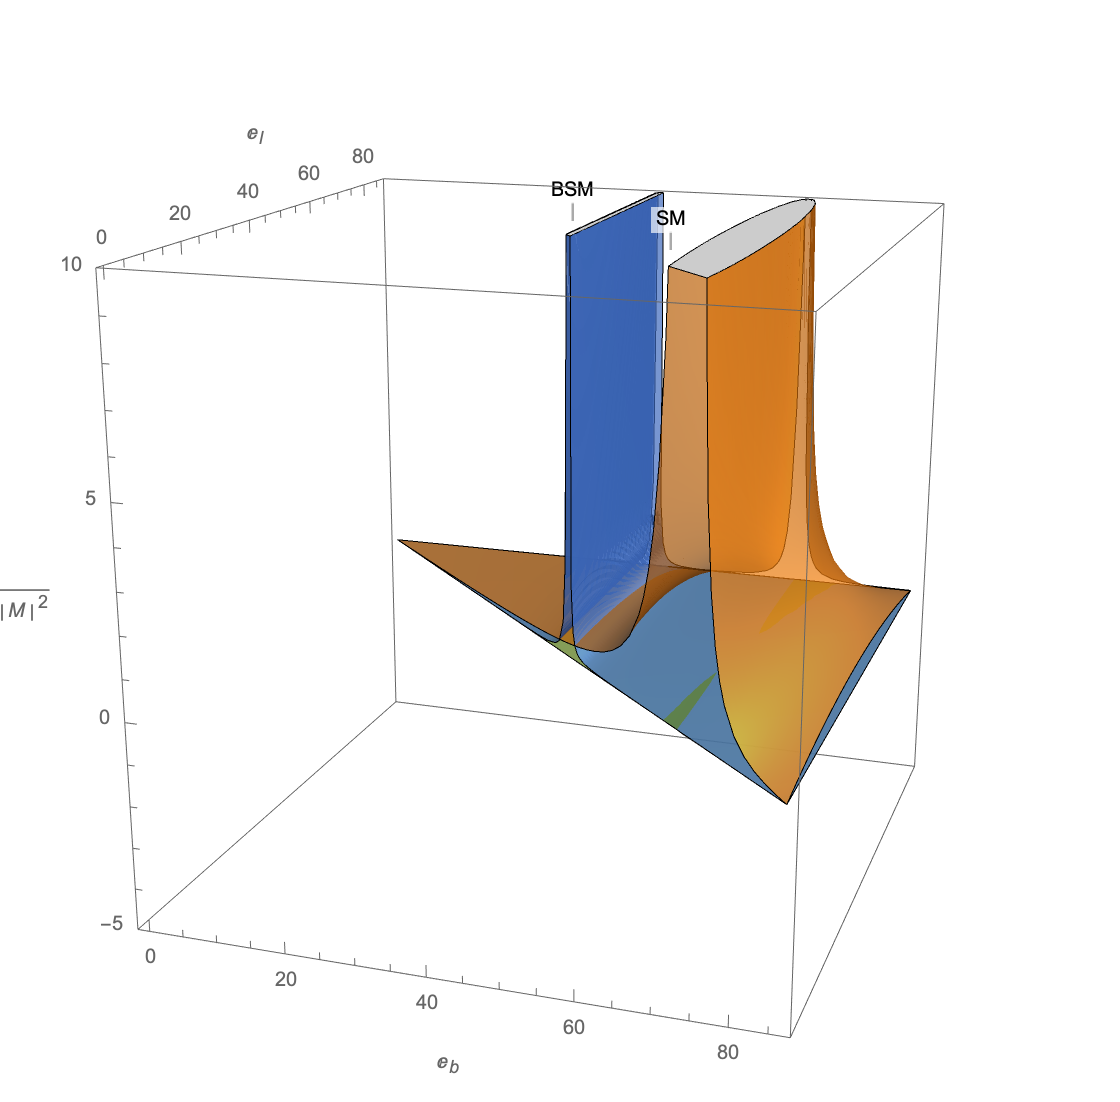
\includegraphics[width=0.4\textwidth]{chapters/RelatedWorks/sectionBSM/figures/2HDM_120_10.png}
    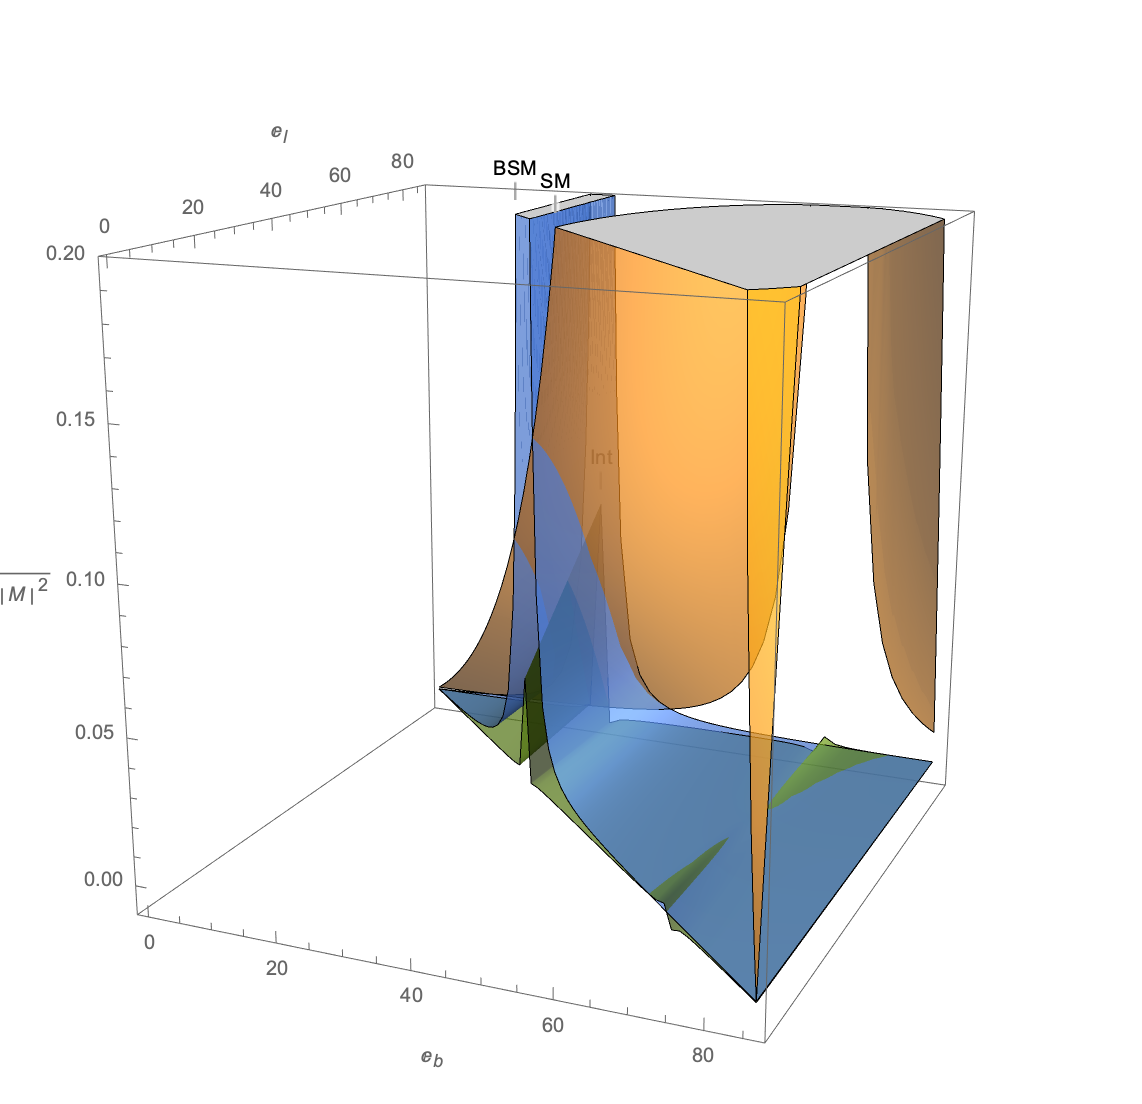
\includegraphics[width=0.4\textwidth]{chapters/RelatedWorks/sectionBSM/figures/zoom_2HDM_140_10.png}
    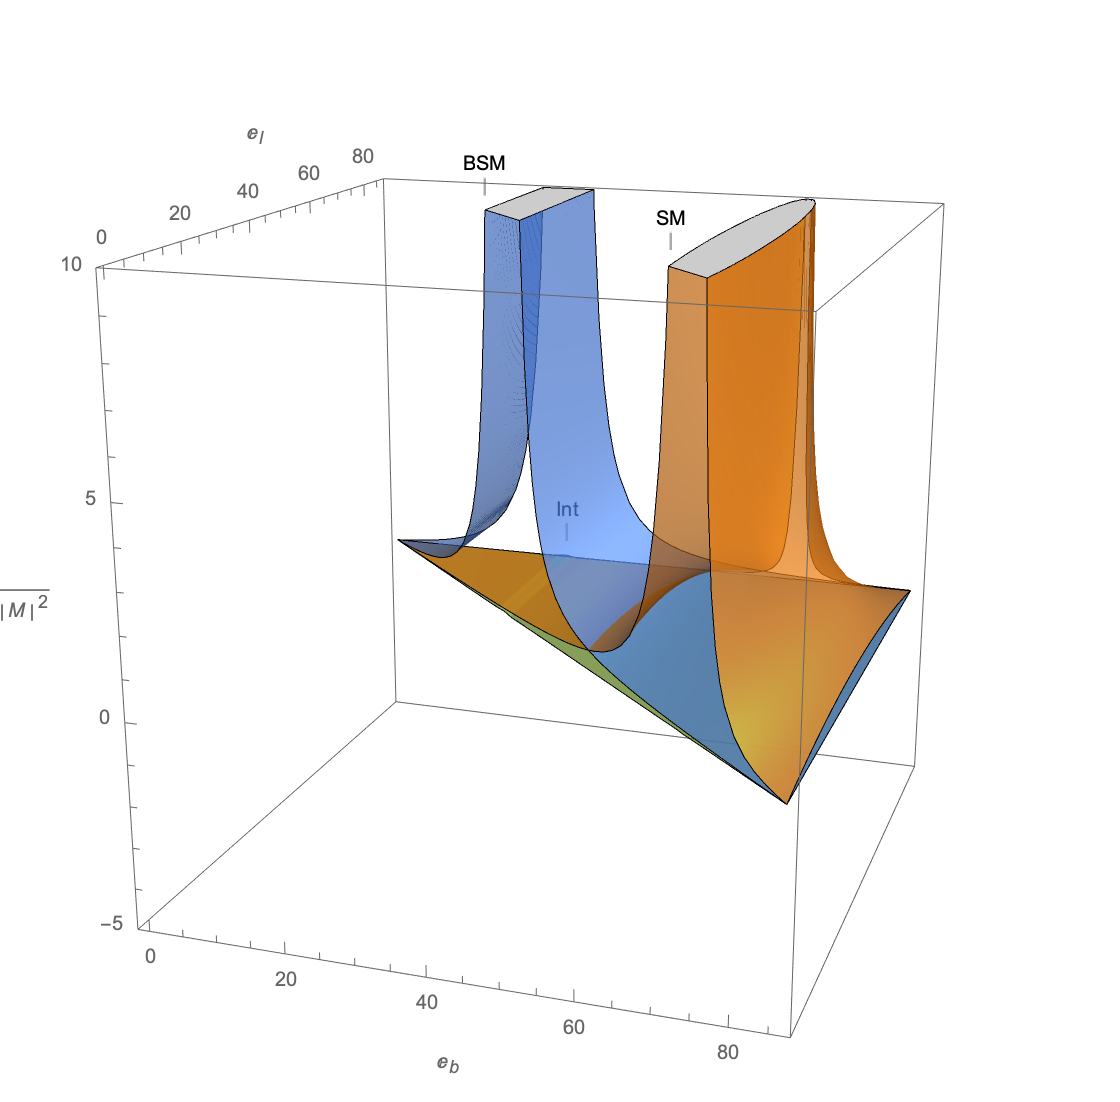
\includegraphics[width=0.4\textwidth]{chapters/RelatedWorks/sectionBSM/figures/2HDM_140_40.png}
    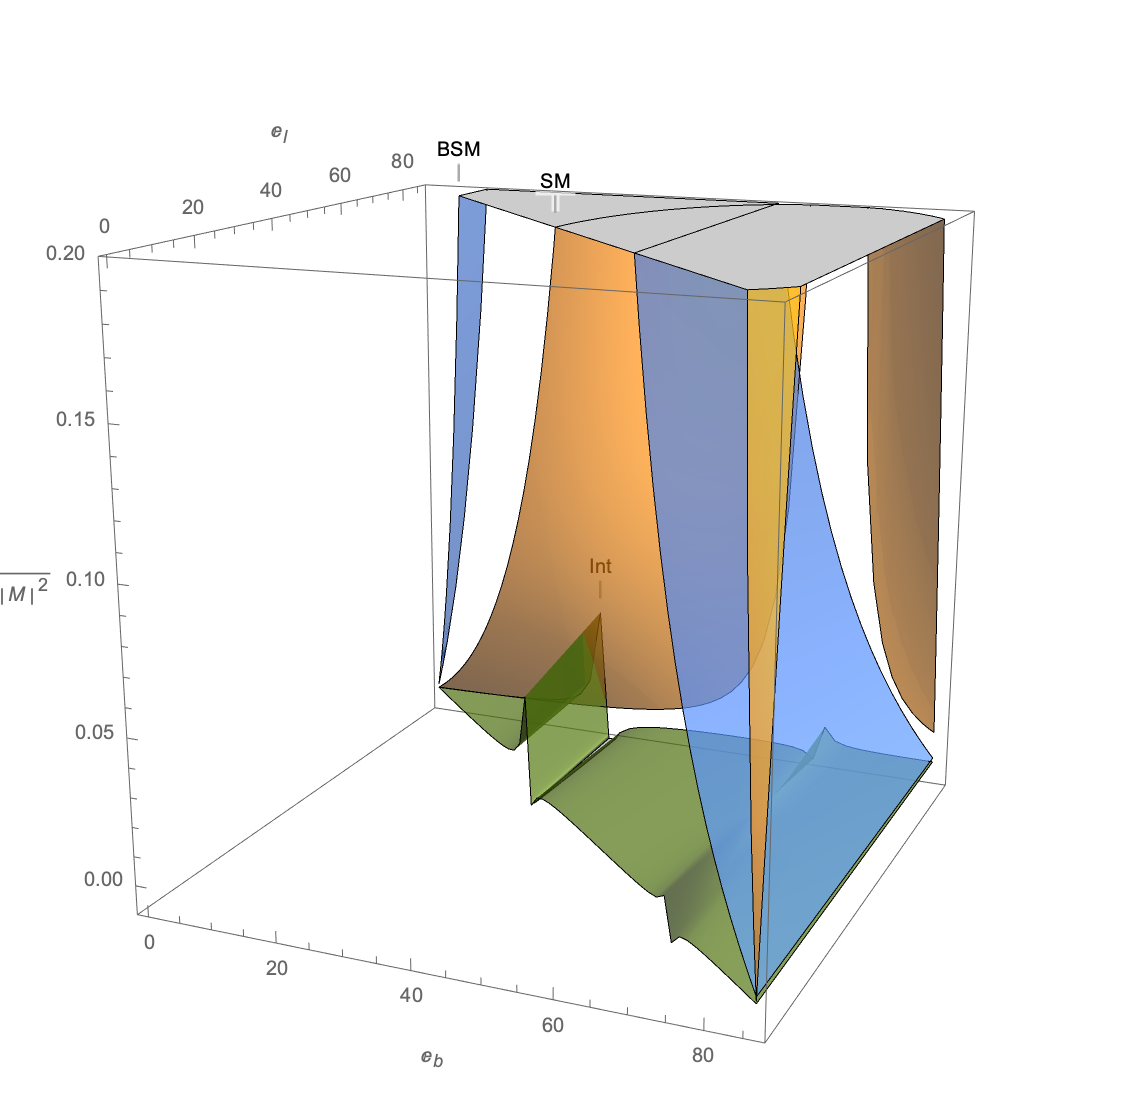
\includegraphics[width=0.4\textwidth]{chapters/RelatedWorks/sectionBSM/figures/zoom_2HDM_140_40.png}
    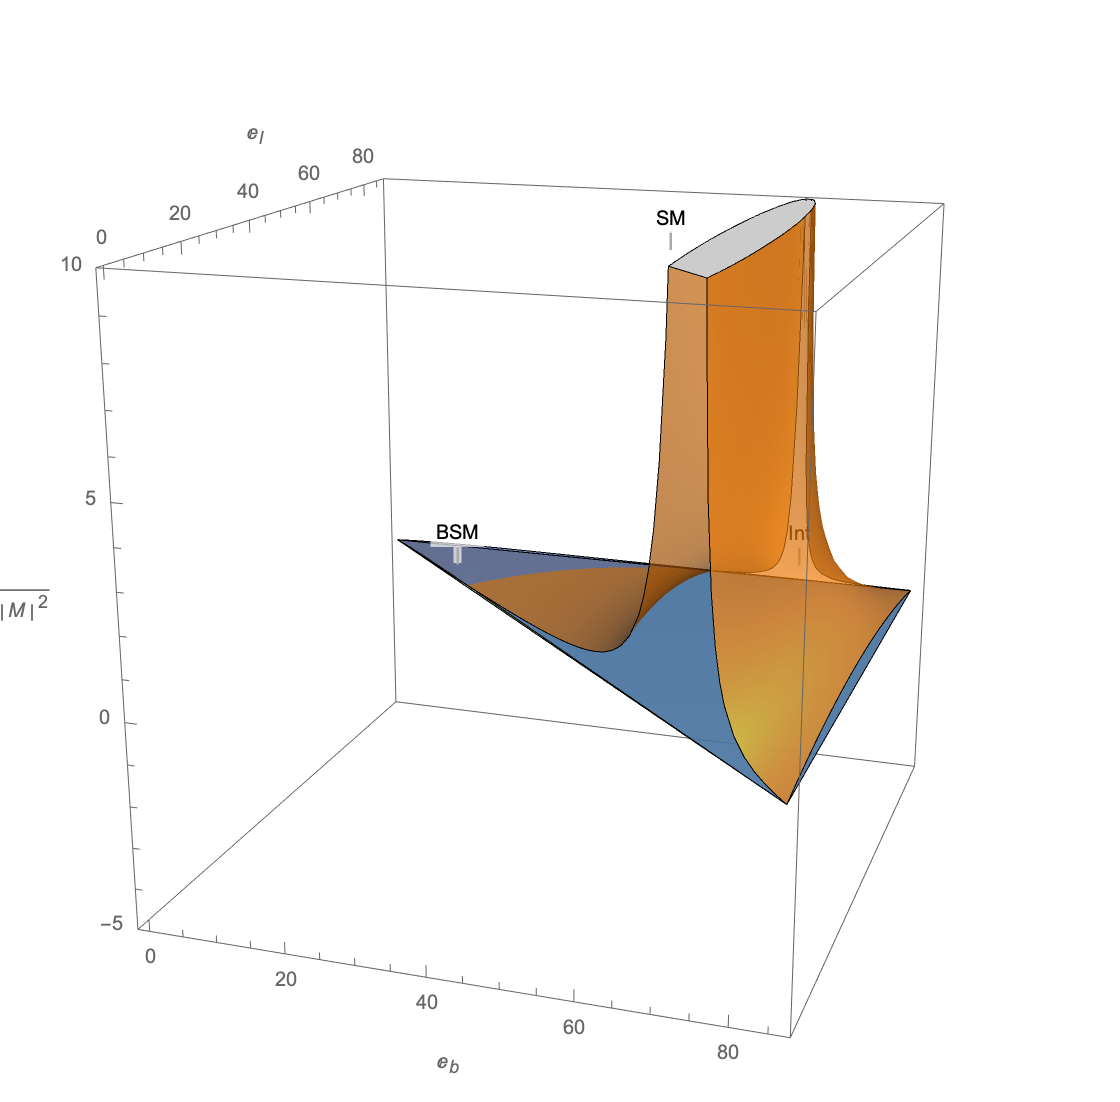
\includegraphics[width=0.4\textwidth]{chapters/RelatedWorks/sectionBSM/figures/2HDM_200_40.png}
    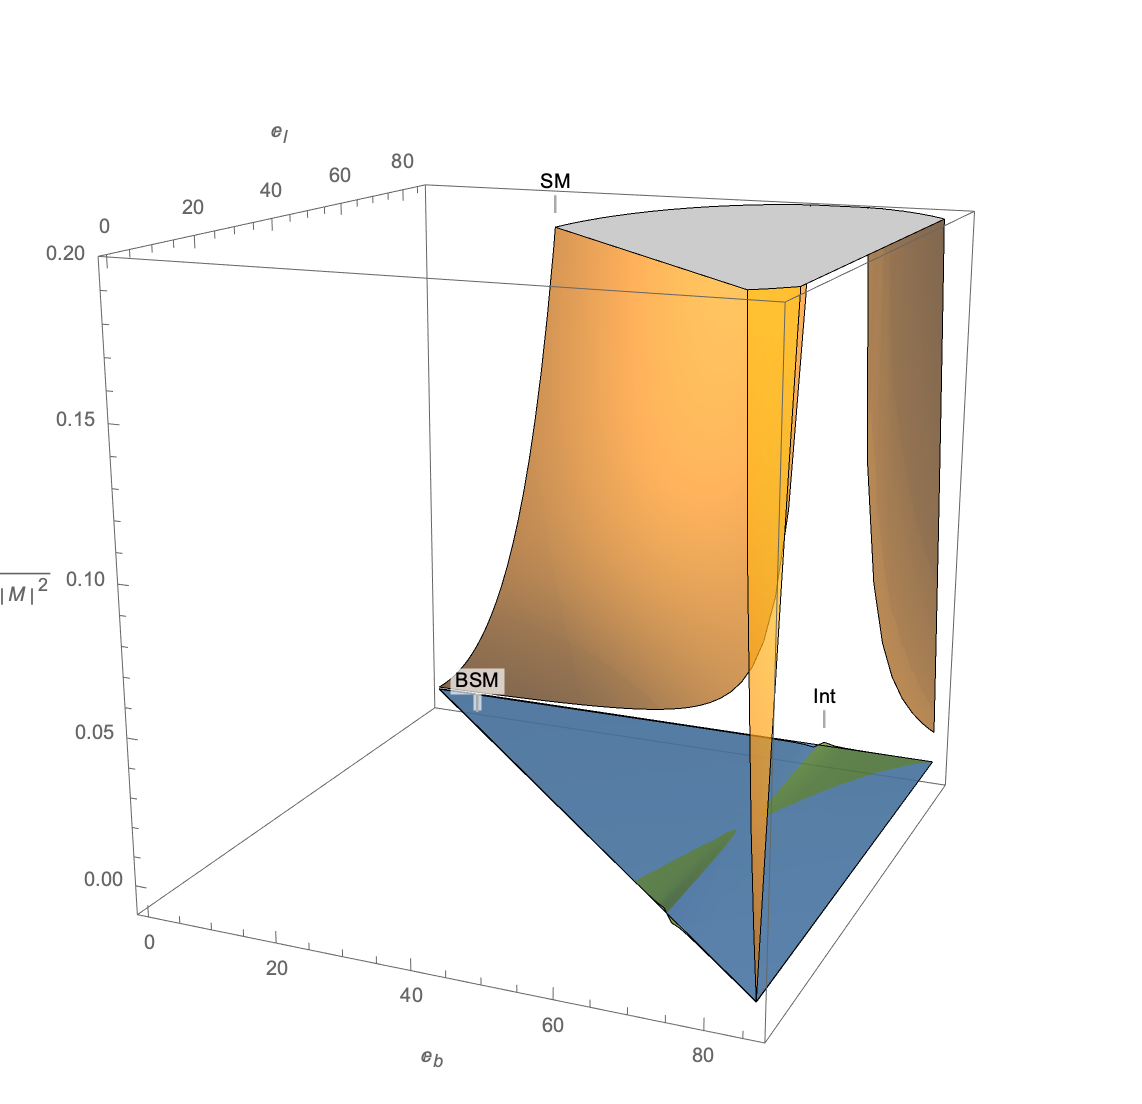
\includegraphics[width=0.4\textwidth]{chapters/RelatedWorks/sectionBSM/figures/zoom_2HDM_200_40.png}
    \caption{  $\overline{ |\mathcal{M}|^2 } _{H}$ and $ \overline{ |\mathcal{M}|^2 } _{int}$ are 2D functions of $(E_1, E_3)$ with two parameters $(m_H, \tan\beta)$. The $\overline{ |\mathcal{M}|^2 } _{W}$, $\overline{ |\mathcal{M}|^2 } _{H} $ and $\overline{ |\mathcal{M}|^2 } _{int}$ are shown as orange, blue and green surface, respectively. The valid kinematics is a triangle area on the $(E_1, E_3)$  plane. The first, second, and third row uses model parameters $(m_H = 140 \text{ GeV}, \tan\beta=10)$, $(m_H = 140 \text{ GeV}, \tan\beta=40)$, and $(m_H = 200 \text{ GeV}, \tan\beta=40)$. The right column is the zoom-in views of the left column to show the small interference amplitude squared $ \overline{ |\mathcal{M}|^2 } _{int}$.}
    \label{fig:relatedWorks:bsm:chargedHiggs:m2}
\end{figure}




Finally, using Equation~\ref{eqn:relatedWorks:bsm:decayWidth}, the extra top width due the BSM $H^+$ equals the integral of  $\overline{ |\mathcal{M}|^2 } _{H} +  \overline{ |\mathcal{M}|^2 } _{int}$
\begin{equation}
	\Gamma^{BSM} = \frac{1}{64 \pi^3 m_t} \int_{0}^{m_t/2} dE_3 \int_{m_t/2-E_3}^{m_t/2} dE_1  \bigg\{ \overline{ |\mathcal{M}|^2 } _{H} +  \overline{ |\mathcal{M}|^2}_{int}  \bigg \},
\end{equation}

\noindent Upon integrating over the triangle area on  $(E_1, E_3)$ plane, we get the BSM effect only depends on the model parameters, $\Gamma^{BSM} (m_H, \tan\beta)$. Take $m_H = 140 $ GeV and $\tan\beta=8$ as an example, $\Gamma^{BSM}= 14.6 \text{ MeV} - 2.1 \text{ keV}$, where 14.6 MeV and  -2.1 keV correspond the  $\overline{ |\mathcal{M}|^2 } _{H}$ and $\overline{ |\mathcal{M}|^2 } _{int}$ integral respectively. When the charged Higgs is  lighter than top quark, the absolutely dominating term is the $\overline{ |\mathcal{M}|^2 } _{H}$ integral and the $W-H^+$ interference effect is neglectable. Take $m_H = 200 $ GeV and $\tan\beta=8$ as an another example: $\Gamma^{BSM} = 0.6 \text{ keV} - 0.8 \text{ keV}$, where the first and second number is from the  $\overline{ |\mathcal{M}|^2 } _{H}$ and $\overline{ |\mathcal{M}|^2 } _{int}$ integral respectively, leading to an ``negative-enhancement'' due to the nature $W-H^+$ interference. When the charged higgs is heavier than top quark, the total BSM effect on the top width is extremely small comparing with the $\Gamma^{SM}= 154 \text{ MeV}$. The relative tau enhancement $\Gamma^{BSM}/\Gamma^{SM}$ can be calculated at different model parameters $(m_H, \tan\beta)$. Figure~\ref{fig:relatedWorks:bsm:chargedHiggs:relEnhance1d} shows  $\Gamma^{BSM}/\Gamma^{SM}$ as a 1D function of $m_H$ for $\tan\beta= 8,20,40,60$, decomposed into $\overline{ |\mathcal{M}|^2 } _{H}$ and $\overline{ |\mathcal{M}|^2 } _{int}$  components. Figure~\ref{fig:relatedWorks:bsm:chargedHiggs:relEnahnce2d} shows $\Gamma^{BSM}/\Gamma^{SM}$ in the 2D parameter space $(m_H, \tan\beta)$. Our analysis confirms the LU (no tau enhancement) with an relative uncertainty of $2\%$ in the tau channel. In  Figure~\ref{fig:relatedWorks:bsm:chargedHiggs:relEnahnce2d}, the contours correspond to 1 and 2 experimental sigma, $\Gamma^{BSM}/\Gamma^{SM} = 2\%$ and $\Gamma^{BSM}/\Gamma^{SM} = 4\%$, are shown as green and blue dash line, the left side of which are excluded by CL 68-95 approximately. Generally, $m_H < 150$ GeV is excluded for all $\tan\beta$ with CL95. But our analysis does not probe the $m_H >m_t$. A direct search with boosted tau is more sensitive to this parameter space $m_H >m_t$. As a comparison, the run-I CMS direct search \cite{Khachatryan:2015qxa} is shown in Figure~\ref{fig:relatedWorks:bsm:chargedHiggs:directsearch}.


\begin{figure}[ht]
    \centering
    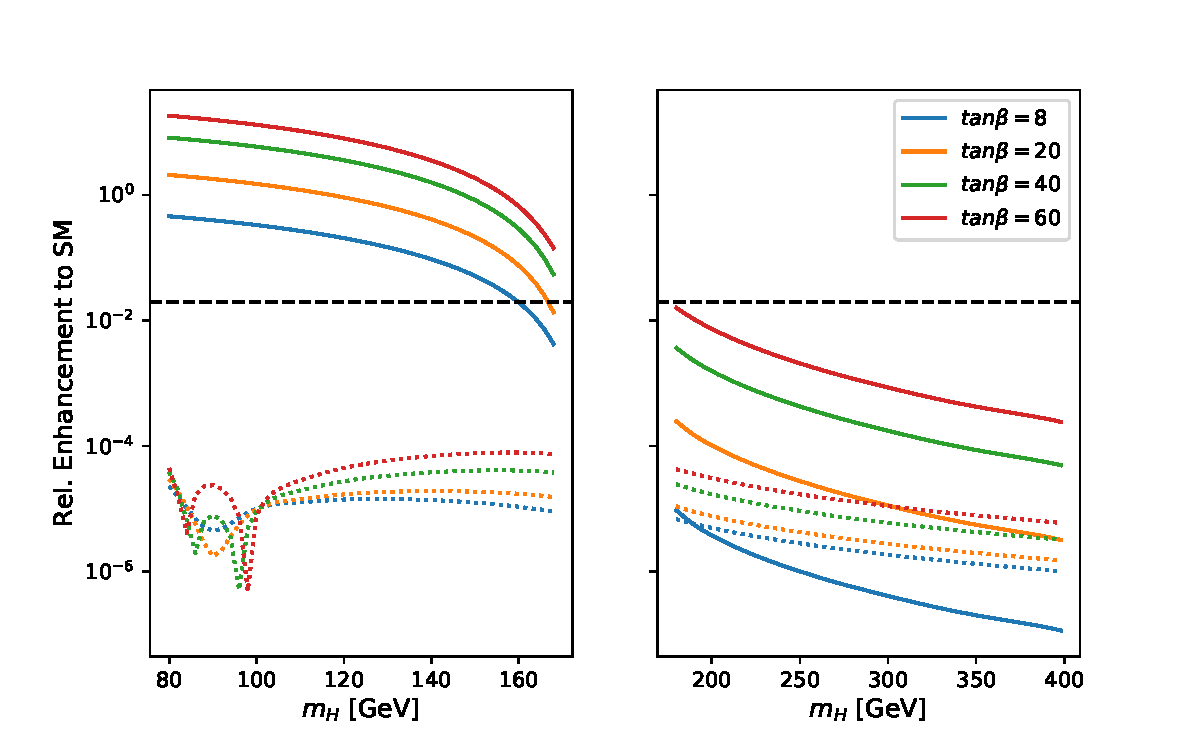
\includegraphics[width=0.89\textwidth]{chapters/RelatedWorks/sectionBSM/figures/RelEnhance2HDM_1d.pdf}
    \caption{ $\Gamma^{BSM}/\Gamma^{SM}$ as function of $m_H$ for $\tan\beta= 8,20,40,60$, decomposed into $\overline{ |\mathcal{M}|^2 } _{H}$ and $\overline{ |\mathcal{M}|^2 } _{int}$  components shown as solid and dash lines. Since $\Gamma^{BSM-int}$ can be negative, its absolute value is taken $|\Gamma^{BSM-int}|$ in this visualization. $\Gamma^{BSM}/\Gamma^{SM}$ in the $m_H>m_t$ is about 2 or 3 order of magnitude smaller than that in the  $m_H<m_t$ region. }
    \label{fig:relatedWorks:bsm:chargedHiggs:relEnhance1d}
\end{figure}







\begin{figure}[ht]
    \centering
    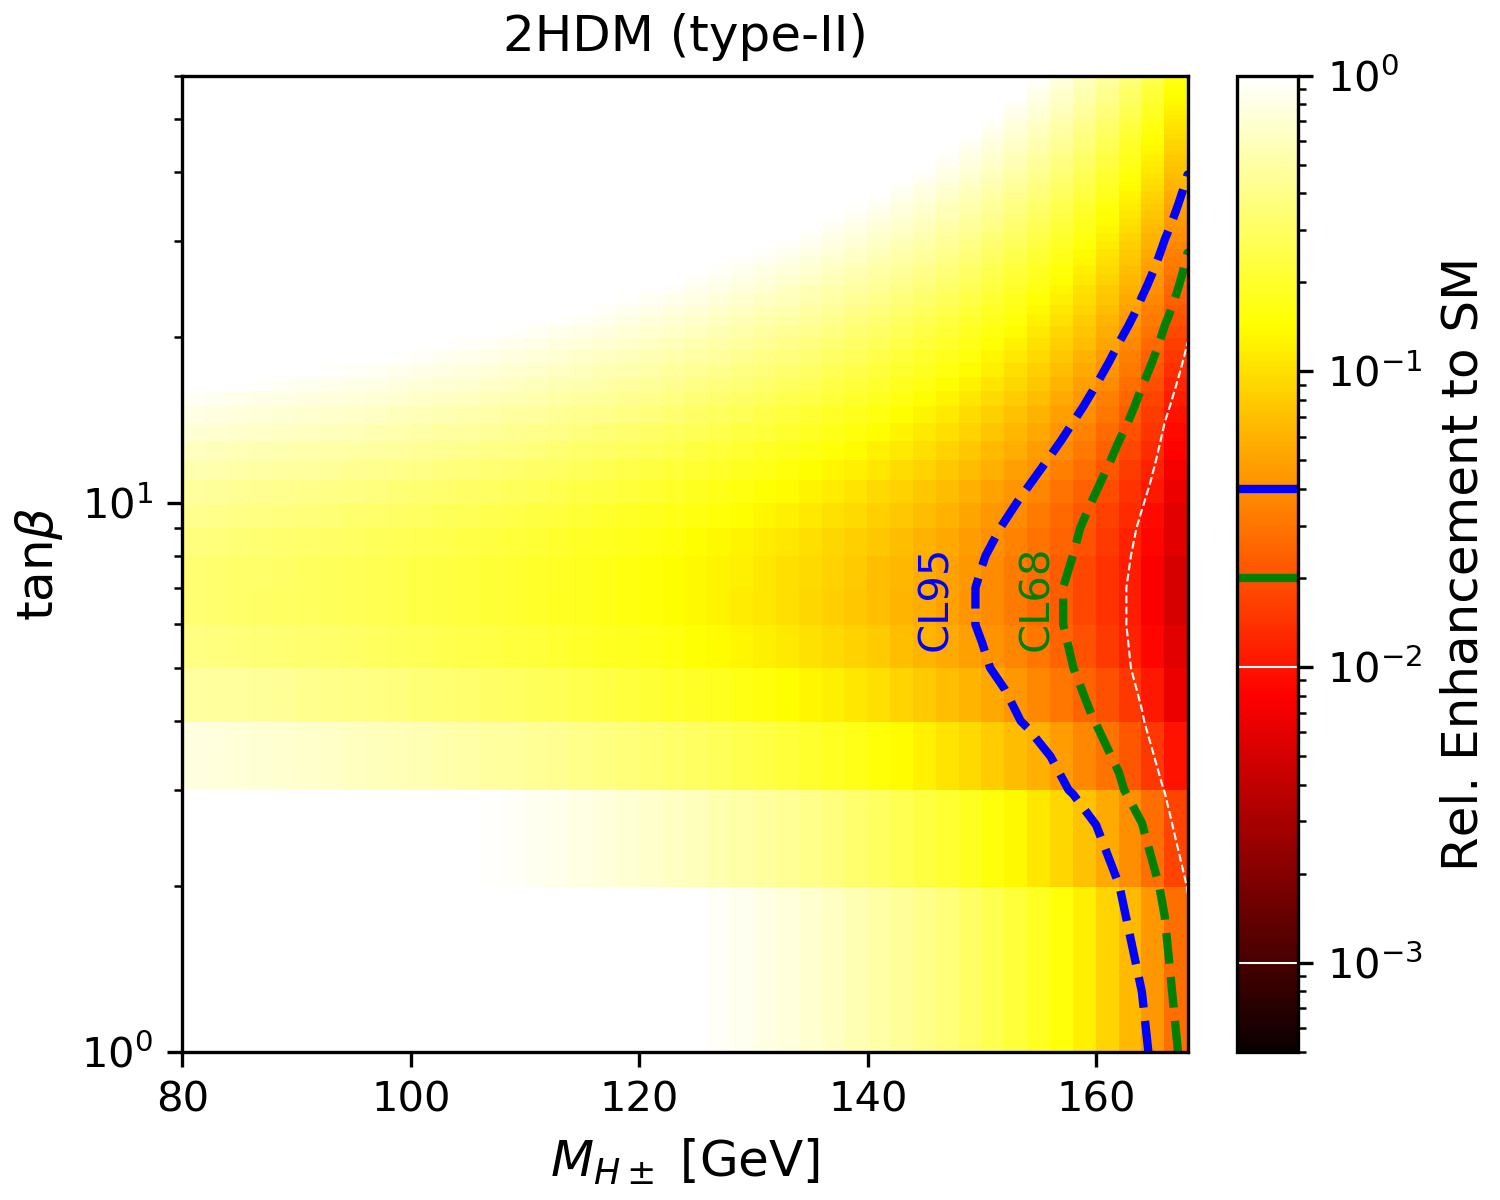
\includegraphics[width=0.49\textwidth]{chapters/RelatedWorks/sectionBSM/figures/RelEnhance2.png}
    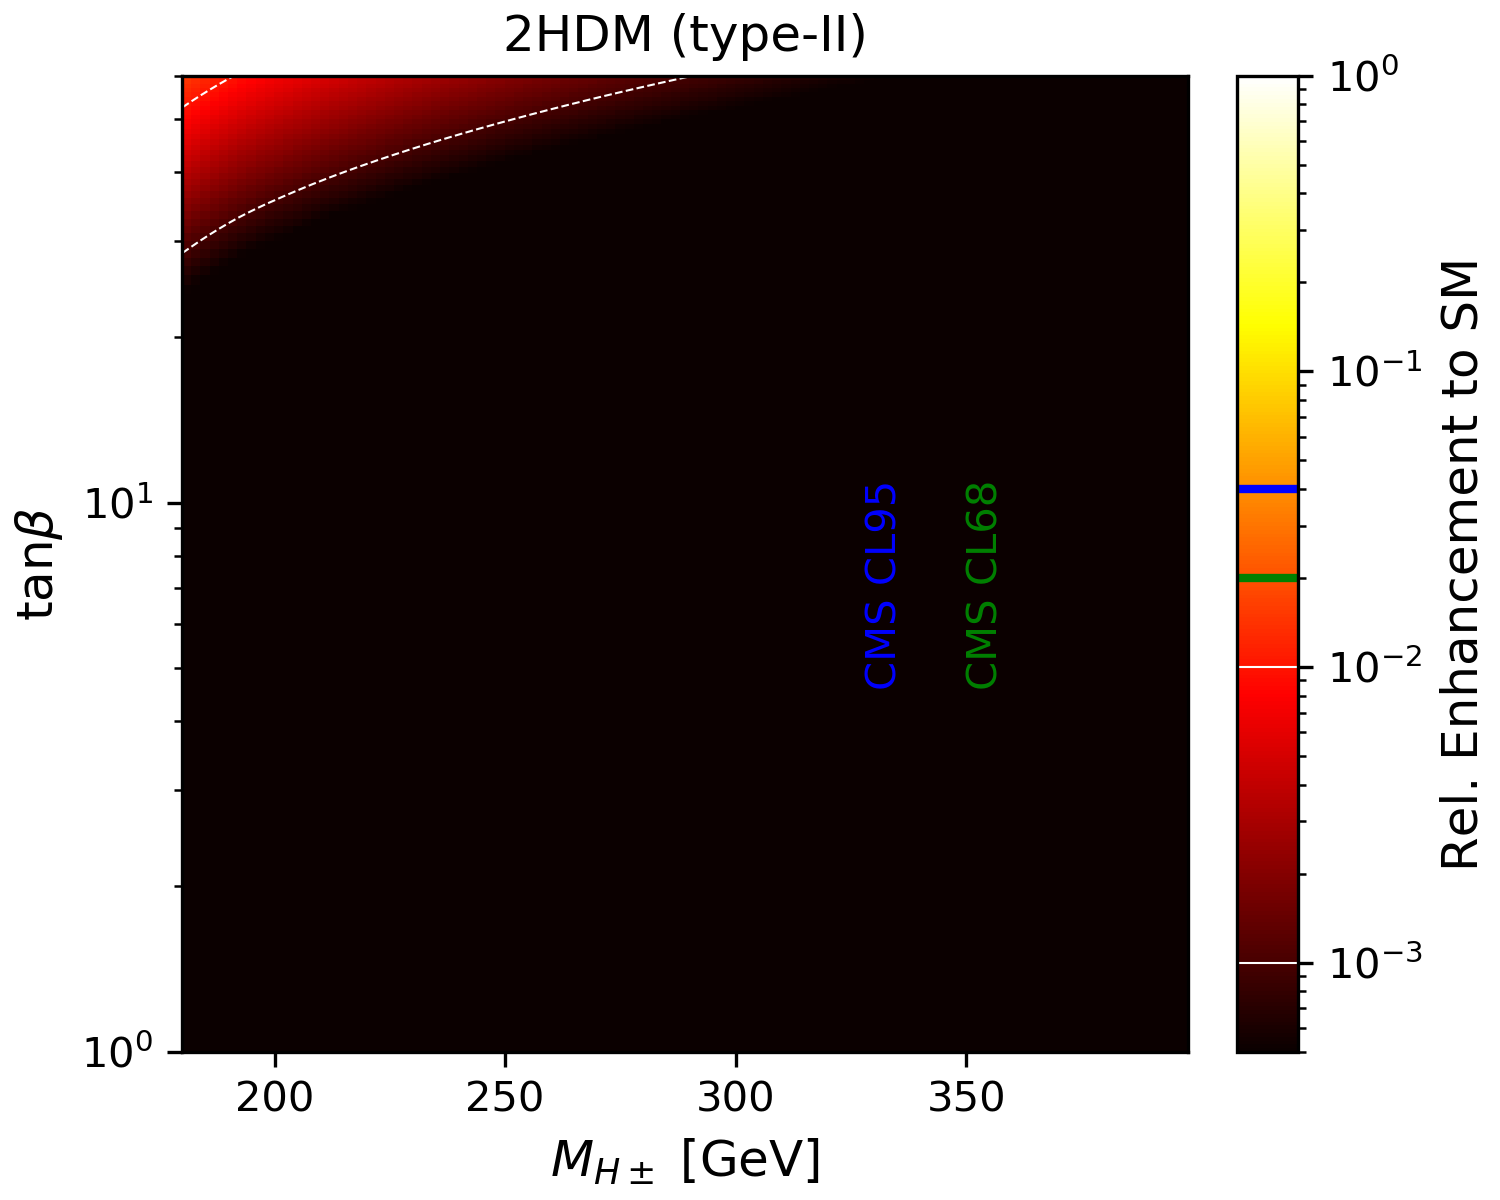
\includegraphics[width=0.49\textwidth]{chapters/RelatedWorks/sectionBSM/figures/RelEnhance2_heavy.png}
    \caption{$\Gamma^{BSM}/\Gamma^{SM}$  in the 2D parameter space $(m_H, \tan\beta)$. Our analysis confirms the LU (no tau enhancement) with an relative uncertainty of $2\%$ in the tau channel. The contours correspond to 1 and 2 experimental sigma, $\Gamma^{BSM}/\Gamma^{SM} = 2\%$ and $\Gamma^{BSM}/\Gamma^{SM} = 4\%$, are shown as green and blue dash line, the left side of which are excluded by CL 68-95 approximately. Generally, $m_H < 150$ GeV is excluded for all $\tan\beta$ with CL95. But our experimental precision does not probe the $m_H >m_t$.  }
    \label{fig:relatedWorks:bsm:chargedHiggs:relEnahnce2d}
\end{figure}

\begin{figure}[ht]
    \centering
    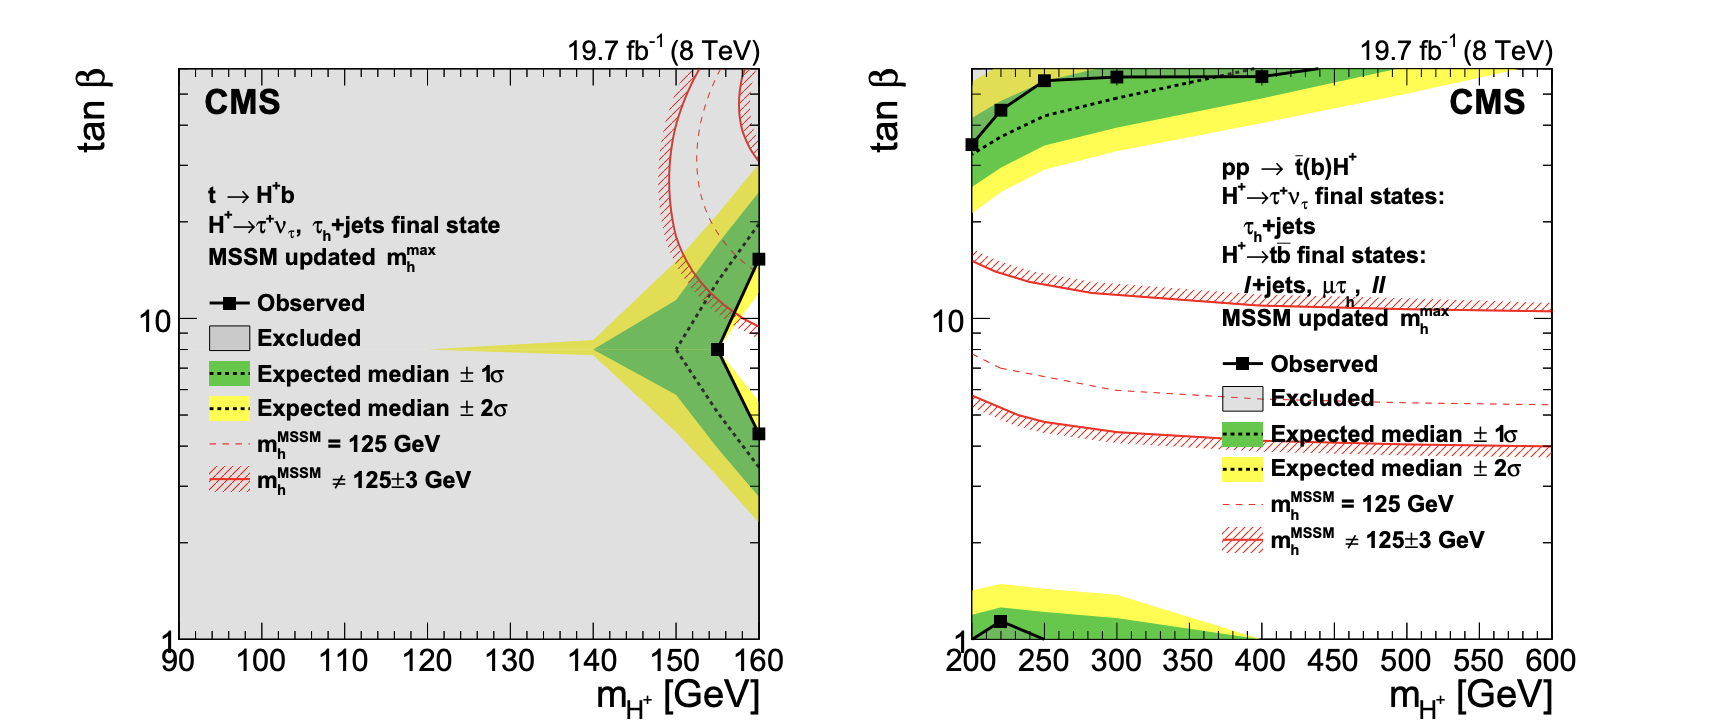
\includegraphics[width=0.9\textwidth]{chapters/RelatedWorks/sectionBSM/figures/2HDM_search.png}
    \caption{Result of the direct search for $H^+$ in the CMS Run-I \cite{Khachatryan:2015qxa}. }
    \label{fig:relatedWorks:bsm:chargedHiggs:directsearch}
\end{figure}



\FloatBarrier

\subsection{Beyond Standard Model with Leptoquark}
\label{sec:relatedWorks:bsm:leptoquark}


Leptonquarks (LQ) is a hypothetical particle with both the lepton number and baryon number, motivated by the GUT and predicted by many theories unifying quarks and leptons. In some GUT, such as Georgi–Glashow SU(5) unification, Pati-Salam model with SU(4) color, leptoquark is a gauge vector boson to mediate forces between the lepton-quark current. In some models, such as extended technicolor models, leptoquark states appear as the bound scalar of techni-fermions. So LQ can be either a scalar or vector boson, which interacts with fermions via $\lambda \cdot (\bar{q} \gamma^\mu l) [LQ]_\mu$ if $s_{LQ}=1$ or via Yukawa interaction $\lambda \cdot (\bar{q}l) [LQ] $ if $s_{LQ}=0$. If the leptoquark couples both to left and right fermions, it is non-chiral. Otherwise, it is possibly couples only to the left- or right-handed fermions and be chiral. There are also possibilities that it couples to only one the fermion family or couples to different fermion families simultaneously. 

There are many direct searches for the leptoquark at the LHC. A pair of leptoquarks can be produced via quark-quark annihilation and gluon-gluon fusion. Meanwhile, single leptoquark production is possible via gluon-quark scattering. CMS and ATLAS have searched leptoquark decaying into the first, second, or third family of fermions. The search with pair production of leptoquarks excludes $m_{LQ}<1.05$ TeV, while the search with single produced leptoquark gives a slightly higher mass limit at 1.755 TeV. 

Besides direct search, leptoquark also causes BSM effective four-point interactions for indirect searches. Search for flavor-changing neutral current (FCNC) puts a strong constraint on the leptoquark that simultaneously involves different lepton generations. Besides, the branching ratio of pion decay into electrons and electron g-2 is also sensitive to non-chiral scalar leptoquarks. Electron-positron collider producing quark pair in the t-channel is also highly constraining the LQ.  Currently, with these indirect limits, it is believed that the leptoquark is more likely to be a chiral scalar or vector coupling to a single family of fermions.

However, it is very model-dependent to the interpreter of our analysis results in the context of LQ. So here, we do not provide a interpretation specific to any LQ models. But in principle, the interpretation could follow the same process as that in Section~\ref{sec:relatedWorks:bsm:WPrime} and \ref{sec:relatedWorks:bsm:chargedHiggs}, where a BSM vector boson and BSM scalar boson are considered as the intermediating propagator.



